%\documentclass[12pt]{scrreprt}
\documentclass[12pt]{report} 

% language may be romanian or english (default is english)
% type may be bachelor or master (default is bachelor)
\usepackage[language=english, type=bachelor]{style}

%\geometry{a4paper,top=2.5cm,left=3cm,right=2.5cm,bottom=2.5cm}
%in style
%controlling the appearance of your headers and footers
\usepackage{fancyhdr}
\pagestyle{fancy}
\lhead{}
\chead{}
\renewcommand{\headrulewidth}{0.2pt}
\renewcommand{\footrulewidth}{0.2pt}

\begin{document}

\specialization{Computer Science}	
\title{Separation of concerns in cross-platform development}					   
\author{Guceanu George - Marian}											
\supervisor{Lect. Dr. Cojocar Dan}				
				
\maketitle


\newpage
\thispagestyle{empty}
\mbox{}
\newpage
\pagenumbering{roman} 

\cleardoublepage


\par
The goal of this thesis is to make an overview of cross-platform development. 
What is the current state of this software development branch, and more importantly what are the main approaches regarding it.
\par
The relevance of this subject is marked by the evergrowing technological advancements.
In the past decade more and more machines and platforms came to life that needed to be interoperable and had to communicate with each other.
This became a necessity especially because all of them brought alongside different operating systems.
\par 
As a consequence, a lot of development platforms were created.
With the increasing relevance for them, more transpositions of the application were needed.
It was inconvenient to use an application that is available for only one platform.
For the software engineers it meant more code bases that needed maintenance and also a lot more learning.
\par
I will analyze the evolution of software development, what it meant along the decades, from the earliest days, up to the starting point of cross-platform development.
This is needed, so we can see the buildup that has been created, turning it into a must-have, rather than a concept.
Further on, I'll make a case for the current state of cross-platform development.
What are the main features it provides, the legacies it kept from it's predecessors, how it is used today and what are the most important tools used.
Then, an analysis over the principle of separating concerns will provide us with the most appreciated features, and see how they align with the needs identified earlier.
I will do a breakdown of this principle, see how it has been approached already and why it is a global standard.
Afterwards, I will make some regards towards the impact this principle provides, by overlooking some metrics that should provide empirical data, according to the provided examples.

\vspace{0.5cm}	
\hrule
\vspace{0.5cm}	
%\cleardoublepage



\tableofcontents


\newpage
\pagenumbering{arabic}

\chapter{Introduction}

%\chapter*{Introducere}
\label{intro}


Cross-platform development is a modern approach to transitive applications.
It is a domain that gained popularity along the years, due to constant innovations in the gadget realm, such as the smartphone, the tablet or the game console.
Each of these took a different approach on their system design or their operating system, hence creating a multitude of "platforms", all with unique features and perspectives regarding development.
\par
This thesis will have \textit{n} main chapters.
In the first one, we will take a look at the history of development as a whole, and see the turns it took along the years.
In this chapter I will also analyze the evolution of computers, from the earliest times until present.
Then I will link this evolution to software development, to see why cross-platform development turned from a very specific niche to an actual problem.
\par
In the second chapter, I will analyze the current state of cross-platform development.
The first subject will cover the lack of separating concerns in this branch.
I will analyze statistics and observe the consistency that has been preserved throughout the years.
Then, the second subject will be what this branch kept as legacy from its parent derivatives.
To be more exact, this will also be divided into three areas of concern: what are the positive features that live on, regarding several aspects such as performance and code maintenance, what are the negative features that continued out of pure legacy and comfort, and also the features that lie in between the ones aforementioned.
\par
Third chapter will contain an overview and a history of separating concerns as a development principle, and also from an architectural point of view.
This will be a thorough analysis over the positive and negative outcomes that separation of concerns can have.
Then I will make a point by point cover over the advantages this principle proposes and see how it aligns with the upgrades that this branch needs.
\par
In the fourth chapter I will go into more details about the separation of concerns principle.
There will be an in-depth approach towards how it is also separated into different notions, layers and practices.
I will then take the already in-use principles of cross-platform development and separate them, so that they will be fitting the aforementioned layers.
\par
Fifth chapter will cover the impacts of separating concerns.
Here I will do a thorough analysis on the theoretical advantages and disadvantages, and then proceed to measure them.
Collected data will sum up to a report that should prove the above points, all within a given metric.
I will analyze code maintainability, reusability, scalability and more, and see the time complexities, measure memory usage, and then present the challenges regarding debugging, tooling and the learning curve.

%\addcontentsline{toc}{chapter}{Introducere}
%\addcontentsline{toc}{chapter}{Introduction}

\chapter{History of cross-platform development}
\label{chap:ch1}

\indent
\par



%\begin{figure}[htbp]
	%\centering
	%	\includegraphics[scale=0.65]{./figures/fig_3_1.eps}
	%\caption{Ciclul de dezvoltare al sistemelor bazate pe componente adaptat modelului cascadã}
	%\label{FigCBSD}
%\end{figure}
In this chapter, I will elaborate on the progresses made throughout the decades regarding designing software and the evolution of hardware, and see how we ended up with cross-platform development as a necessity.

\section{The 1940-1970 timeline}

\subsection{The 1940's}

\par

During this decade, the "Big Bang" happened.
John Mauchly and Presper Eckert, designed and built the "first digital, electronic computer"\cite{eniacHistory} and came up with the legendary ENIAC.
A computer that was designed with a military goal in mind.
ENIAC was developed at the University of Pennsylvania, being funded by the U.S.
Army, mainly because the teams at the other Universities were not able to keep up with the Army's needs for computing artillery firing tables "for the war 
effort".\cite{eniacDesign}

\par
This computer revolutionized computations as it was the first machine to ever allow any kind of stored procedures, by introducing plugboard wiring and portable function tables in favor of the previous punch cards.
Plugboards were connecting switches, which were "capable of storing one complex instruction for the use of the accumulator".\cite{eniacSwitches}
This meant that, the entirety of the computation was digital, and reconfigurable.
Unfortunately, it also meant that, between each run or change, the computer had to be shut down so the wiring could be redone.
\begin{figure}[htbp]
    \centering
    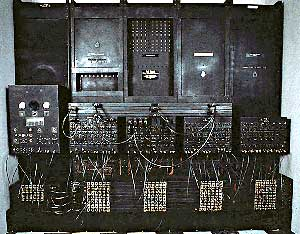
\includegraphics[scale=0.5]{pictures/ENIAC_plugboard_switches.jpg}
    \caption{ENIAC plugboards and switches}
    \label{eniacPlugboardSwitches}
\end{figure}
\par
But, even so, a good algorithm structure was needed, that being mainly because 'these architectural differences lead to some differences in the approach needed for programming'\cite{eniacDesign}.
So the operators of the machine came upon some design and operation principles, that are still observable in the modern world, such as 'Dataflow', 'Parallelism' and 'Looping and branching' \cite{eniacDesign}


\subsection{The 1950's}
\par
Software engineering and designing became a subject of discussion as early as the 1950's.
During those days, this terminology meant something entirely different than what we know of today.
The quote that depicted it quite accurate is: `\textit{Software engineering is like hardware engineering}`\cite{boehmb06}.
This is mainly because software was regarded as building a machine: you embody a plan, manually check it and then get it running on the computer.
\par
The biggest invention of this decade was the concept of storing, organizing and manipulating data.
It is during these times that it got a name, "data processing"\cite{firstDBMS}.
It is also now when the storage, retrieval, and updating of data has been a "key requirement for most computer applications"\cite{firstDBMS}.
These are things that followed up and evolved into the modern world, and they can be observable as most up-to-date applications require enormous data volumes.
Data started to play an important role.
It was regarded as one of the building blocks of applications back then.
This is also another pattern that is kept into the modern development world.
\par
In this same decade, more specifically in 1952, the first compiler was made, for the A-0 system.
This compiler was introduced and put into practice by one of the founding figures of the programming field, that being Grace Hopper.
This represented a turning point, as she proved that computers should understand "human-like" languages\cite{a0compiler}, not the other way around.
Now the tool of software became a much more teachable subject, and had the potential of turning to be more at-hand for everybody.
In 1953 she developed A-2, which is considered to be the first open-source piece of software ever.
That is due to the fact that its source code was given to the customers and they were encouraged to send in possible improvements.


\par
The first commercially-available compiler was put on the market not that later on.
It is the FORTRAN, "formula translator"\cite{a0compiler}, compiler that was developed by IBM in 1957, for the 704 computer.
It is now that we can see a mould for software.
During the same decade, the first pieces of both open-source and closed-source software were developed and put on the market.



\subsection{The 1960's}
During this time period, the machines got a bit more user friendly and code became easily replaceable.
This turned software into something far different to hardware.
COBOL is now introduced to the market, and it made a case for itself.
It is the first programming language that was considered easy to use and read, and that introduced the concept of machine abstraction.
This meant that it did not require a dedicated machine to run.
It was, in a very abstract and distant way, the first piece of cross-platform software.

\par
Now, the ability to rewrite code enabled developers to turn towards a "code and fix" approach\cite{boehmb06}.
This meant that coding was something that did not require as much manual calculations, and that can be thought of and corrected along the way.
Not only that, but it is the first time during this decade that a problem was eradicated: having exact hardware in order to collaborate on development.
This is considered to be a menial job for the modern programmers, but during those times it was a long due issue.
\par
This is one of the biggest turning points in software design, as it allowed for a practice that is still put to good use today.
Correction of code, be it from a logical or opinionated point of view, during development lead to branching and forking, tools that are still used in modern development.



\section{The 1970 - 1990 timeline}
\subsection{The 1970's}
This decade is perhaps the most important step in software development.
This is the decade that made modern computing the thing that we know and love.
In 1972, Dennis M.
Ritchie and his team created the C programming language.
To say it was revolutionary, was an understatement.
This project turned Dennis Ritchie into a titan and unforgettable figure of the software world.
He was a "bearded, somewhat disheveled computer scientist"\cite{ritchieJobs} that stays at the foundation of the things we make most use of today, for exmaple the internet.

\begin{figure}[htbp]
    \centering
    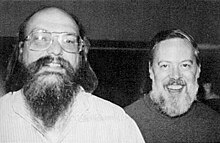
\includegraphics[scale=0.7]{pictures/KenThompson_and_DennisRitchie1973.jpg}
    \caption{Ken Thompson and Dennis Ritchie, 1973}
    \label{unixMakers}
\end{figure}

\par
C is a language that derived from BCPL (Basic Combined Programming Language).
It became relevant when, yet again, Dennis Ritchie decided to use it in order to re-write the source code of the UNIX operating system.
Such and operation was deemed necessary by him mainly because the U.S government categorized the capitalism of such a product as a violation the "Sherman Antitrust Act"\cite{unixRepo}.
Due to this, AT\&T released the Operating System as royalty-free, but later however licenses became a bigger obstruction, hence the limitations in the access of the source code.
Then Dennis Ritchie decided to re-write the whole OS in the high-level programming language in C, in 1973.
This project, although later forked into many other operating systems such MacOS or GNU/Linux, was maintained and developed up to this day to the FreeBSD project.
A part of the legacy assembly source code of UNIX is still on GitHub, at the repository 'dspinellis/unix-history-make'.

\begin{figure}[htbp]
    \centering
    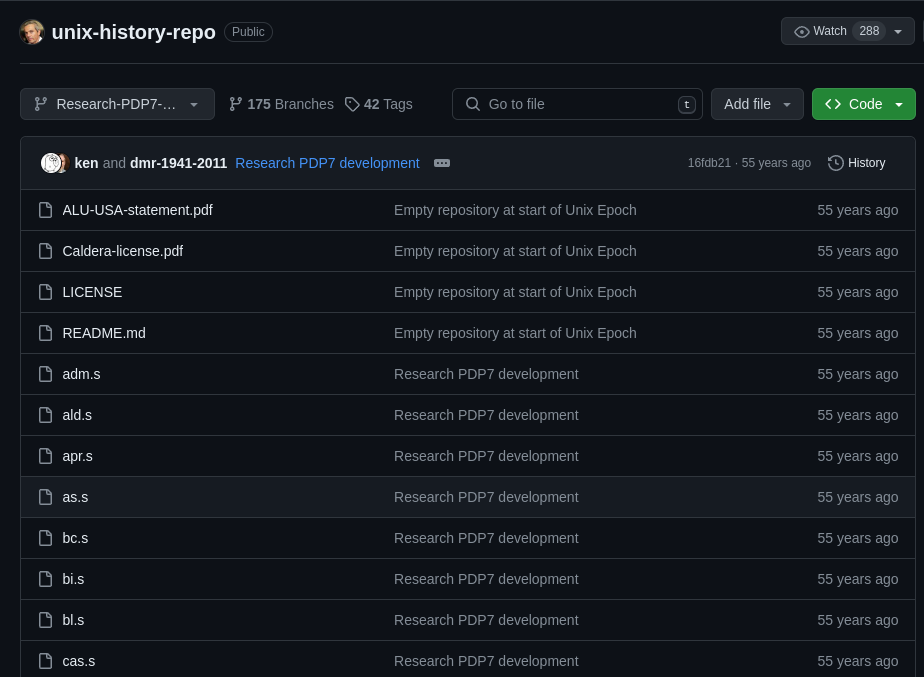
\includegraphics[scale=0.5]{pictures/unix_repo.png}
    \caption{TODO:change to white theme Repository containing the assembly source code of UNIX}
    \label{unixRepo}
\end{figure}


\subsection{The 1980's}
During the 80's, software design became an area on interest for most people involved in the computer science field.
One of the earliest approaches of software design is the Layered architecture.
This was firstly introduced as a need because of the way computer networks were operating.
Now, files were getting bigger and because of that, "The programmer must maintain descriptions of
how various alternative designs are distributed among files"\cite{layeredArchitecure80s}.

\par
Along with these software design paradigms, this decade introduced the first implementation of a version control system.
It worked quite similarly to the modern approaches.
It stored the differentials of the files in a 'delta' file\cite{layeredArchitecure80s}.
This file was one of the deterministic factors for which version control and layered architecture were introduced.
As files grew bigger in size, the delta file associated with it was also getting clunkier, thus making reverting or alternating changes a time and memory-consuming task, and by separating the files into smaller ones, each depending on the other one, this process would be optimized.

\par
This decade brings the most enhancing and used tool of the modern world, the internet.
Although it is believed that invented rather earlier, in the late 60's, it is in 1983 when ARPANET and DDN (Defense Data Network) switched to the TCP/IP standard, "so that computers of many kinds could communicate with each other, no matter what kind of network they were connected to in the Internet".\cite{arpanetDdn} This was a big leap, as ARPANET was an already enormous cluster of interconnected computers, therefore the computers entering the network would have access to them.

\begin{figure}[htbp]
    \centering
    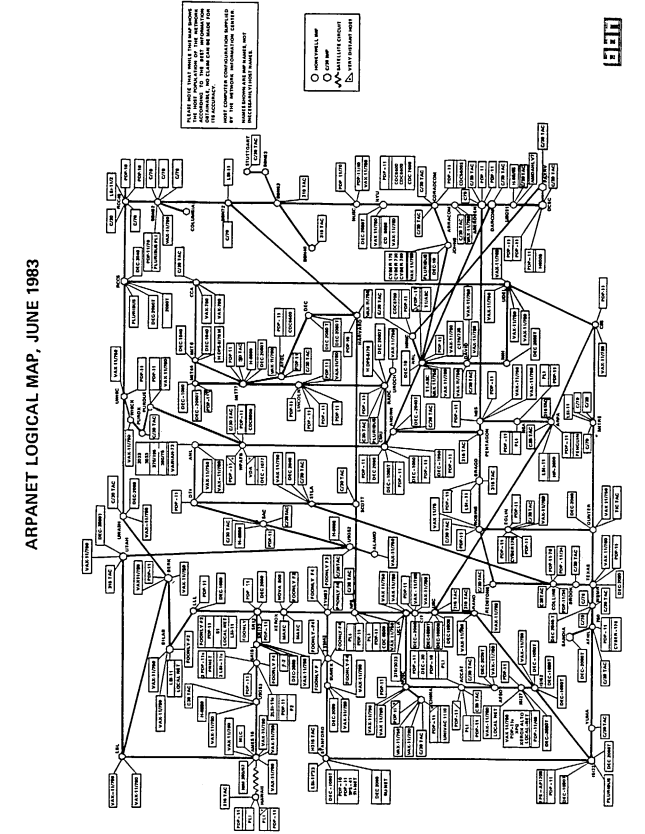
\includegraphics[angle=270,scale=0.35]{pictures/arpanet.png}
    \caption{ARPANET logical map, 1983}
    \label{arpanetLogicaMap}
\end{figure}


\par
Due to this, a doubling of household computers happened until the 90's.
This meant that more people were put on the network, and, due to this, all the computer owners had access to each other's data and information, should they wanted to access it.

\begin{center}
    \begin{tabular}{|| c | c ||}
          \hline
          \textbf{Year} & \textbf{Percentage} \\
          \hline
          1980 & 2.8\% \\
          \hline
          1982 & 6.2\% \\
          \hline
          1983 & 7.3\% \\
          \hline
          1984 & 8.4\% \\
          \hline
          1986 & 9.5\% \\
          \hline
          1988 & 12.5\% \\
          \hline
          1989 & 15.0\% \\
          \hline
    \end{tabular}
\end{center}

\par
As you can see, the biggest jump in the percentages happened between 1980 and 1982.
But, since ARPANET switched their protocols in 1983, the number of computers in personal households has grown by a staggering 7.7\%, a bit more than double.



\subsection{The 1990's}
This decade has been the most influential one for the modern world, and especially for the computing area.
With the evergrowing increase in computer-owning households and the creation of the internet, we see how this affected the development process, thus leading to a series of projects that are major key-factors in our current timeline.

\par
In 1990, we see the first true creation of cross-platform software.
At CERN, Switzerland, Tim Berners-Lee submits two ideas for what should be the Web, back in March 1989.
Until the Christmas of 1990, he contoured the World Wide Web, making the first prototype for it.
The intention of this project was to be "a pool of human knowledge", thus allowing for ease of communication between people who were geologically disjointed\cite{worldWideWeb}.

\par
This project offered features that are still generally available today, such as a server, HTML, the first web programming language, URL's and the first browser.

\section{The 2000's}
\subsection{First definition}
Now, during this decade we can see some of the first mentions of the term "cross-platform development".
That is due to the fact that more and more "platforms" (example: Windows, MacOS) started rising and gaining popularity, and certain large applications needed to behave and act accordingly on all of them.
I will refer to "platform" from now on as development environments, for example Android meaning not only the mobile phone operating system, but also the ecosystem surrounding it, such as smartwatches or TV's.


\par
Some of the first people that proposed this terminology were Bishop J.
and Horspool N., who also gave the first definition to this development branch.
They described the product of it as "software that exists in different versions so that it is available on more than one platform"\cite{firstDefinition}, all the way back in 2006.
In this definition, their meaning of platform is the same as the one I mentioned earlier, because back then the definition was a bit more general, such as "language, operating system, computer, or some combination".
In the same time-period, the Web was starting a world-conquering journey.
Along with it, it brought a whole toolkit of development principles and design patterns, with component-based development being the most praised one.
This is also mentioned and observed by the aforementioned authors, whom agree that component-based development  has made a good impact  toward satisfying "both parts of the definition."\cite{firstDefinition}
\subsection{First toolkits}
The idea of cross-platform development was initially brought as a fix for one of the bigger issues developers faced at the time, and that is building graphical user interfaces (GUI's).
This in itself represented a dilemma because for every platform there were dedicated tools and specific programming languages, for example for Windows there was exclusively .NET with the C\# programming language.
This inherently meant that there was no uniform way of developing such GUI's across platforms.
There is also acknowledgement in this, starting with the earliest days.
Due to such history, there came the stigma that cross-platform toolkits are "integral to GUI development"\cite{firstDefinition}.

\par
Because of this, we can also observe the rise in popularity of some toolkits that were not very seriously taken considered before this realization, such as Qt or GTK+.
These are some of the first cross-platform frameworks that are still used today at a production level, and we can see them used in many well-known applications, such as Spotify for Qt, or the GNOME desktop environment for GTK+.
They are trying to achieve different goals, but one thing that they have in common is that both Qt and GTK+ define a collection of widgets that should work as "platform independent"\cite{firstDefinition}.
This then allowed for the developers to apply a "learn once, code everywhere" approach.

\chapter{Separation of concerns}
Now that we got to understand the origins of cross-platform development, I believe it's time for a move that's just as important for the thesis.
During this chapter, I'll take a step towards a different direction.
I'll take a look at the definitions, because there will be multiple, history, use cases, advantages and disadvantages of the principle of separating concerns.
We'll compare and analyze the views regarding this topic, see where it originated (or all the places of its origins), 
check out what caused it to come into existence, and then do a thorough analysis regarding the benefits it provides, and the disadvantages they bring.


\section{Rise in popularity}
The adoption of the principle of separation of concerns gained significant momentum during the late 20th century and continued into the early 21st century.
While it's challenging to pinpoint an exact time period for its increased adoption, 
we can identify key phases when the concept became more widely recognized and discussed:
\par
During the emergence of object-oriented programming (OOP) in the late 1970s and 1980s, the principles of modularity and separation of concerns gained prominence.
Languages like Smalltalk and Simula popularized OOP concepts such as encapsulation, inheritance, and polymorphism, which inherently promote the separation of concerns.
This period laid the groundwork for the widespread adoption of modular design principles.
\par
The 1990s saw a proliferation of publications and discussions on software design principles, design patterns, and best practices.
Influential works such as "Design Patterns: Elements of Reusable Object-Oriented Software" by the Gang of Four (Erich Gamma, Richard Helm, Ralph Johnson, John Vlissides) were published in 1994.
This book cataloged common design patterns, many of which emphasize separation of concerns.
The 1990s also witnessed the rise of agile methodologies and the growing importance of modular design in software development.
\par
In the early 2000s, there was a continued focus on modular design principles, particularly within the context of domain-driven design (DDD) and agile software development.
Eric Evans' book "Domain-Driven Design: Tackling Complexity in the Heart of Software" (2003) emphasized the importance of separating concerns within a software system to improve maintainability and alignment with business requirements.
This period saw an increasing recognition of separation of concerns as a fundamental principle in software architecture.
\par 
From the mid-2000s to the present day, separation of concerns has remained a central tenet of software engineering practices.
The advent of microservices architectures, cloud computing, and DevOps practices further underscored the importance of modular design and loose coupling.
Additionally, the proliferation of open-source software projects and collaboration platforms facilitated the exchange of knowledge and best practices related to separation of concerns.
\par
Overall, while separation of concerns has been a guiding principle in software engineering for several decades, its adoption 
and recognition as a fundamental design principle gained momentum during the late 20th century and continue to shape software development practices today.
The most significant publications about separation of concerns were written during the 1990s and early 2000s, 
coinciding with the emergence of object-oriented programming and the proliferation of design patterns and agile methodologies.


\section{Definition}
Separation of concerns is a design principle in software engineering where different parts of a system are divided to handle different responsibilities.
This makes the system easier to understand, maintain, and modify because each part focuses on a specific aspect of functionality, 
rather than trying to handle everything at once.
It is a fundamental principle in software architecture that promotes modularity, maintainability, and scalability, or, as Harold Ossher and Peri Tarr put it, 
it's something that stands at the "core of software engineering" \cite{definitionSOC}.
\begin{figure}[htbp]
    \centering
    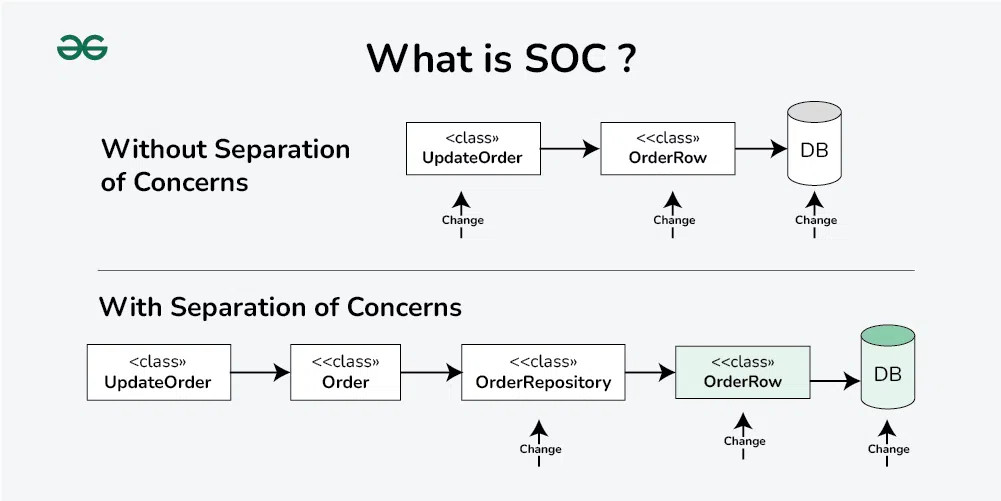
\includegraphics[scale=0.4]{pictures/soc_definition_example.jpg}
    \caption{Separation of concerns definition example, source: \href{https://www.geeksforgeeks.org/separation-of-concerns-soc/}{GeekForGeeks}}
    \label{arpanetLogicaMap}
\end{figure}
\par
Now we'll take an in-depth look at the founding ideas that are holding this principle high in its regard.
These are: modularity, flexibility and reusability, testing and scalability.
We'll take each of them apart and see what they can provide for us.


\subsection{Modularity}
Separation of concerns promotes modularity, where a system is divided into smaller, independent modules.
Each module encapsulates a specific aspect of functionality.
For example, in an application that requires extensive security, 
advanced separation of concerns allows for building mechanisms that "can be merged into the system in a flexible way" \cite{socExample}.
\par
Modularity encourages encapsulation, which involves bundling related functionality and data into cohesive units called modules.
Each module represents a self-contained unit of code that hides its internal implementation details from the rest of the system.
This encapsulation fosters information hiding, reducing dependencies between modules and promoting loose coupling.
\par
Modular design emphasizes defining clear and well-defined interfaces for communication between modules.
These interfaces specify how modules interact with each other, providing a contract that ensures consistent behavior and interoperability.
By adhering to these interfaces, developers can swap out implementations or extend functionality without affecting other parts of the system, as long as the interface remains unchanged.
\par
Modularity allows for varying levels of granularity in module design.
Modules can be large or small, depending on the complexity and scope of the functionality they encapsulate.
Decomposing a system into smaller, more manageable modules facilitates better organization and promotes code reuse.
However, it's essential to strike a balance between granularity and cohesion to avoid overly fragmented or tightly coupled modules.
\par
Overall, modularity is a key aspect of the separation of concerns principle that promotes the organization, maintainability, and extensibility of software systems.
By breaking down a system into modular components with clear interfaces and well-defined responsibilities, developers can create more flexible, scalable, and reusable codebases.


\subsection{Readability and Maintainability}
By separating concerns, the code becomes easier to read and understand.
This is important, becuase it was proven by Raymond P. L. Buse and Westley R. Weimer that 
"low readability correlates more strongly with this direct notion of defect density" \cite{readabilityMaintainability}.
Developers can focus on one aspect of the system at a time, making it easier to debug, maintain, and modify without affecting other parts of the system.
This also facilitates collaboration among team members, as each person can work on different modules independently.
\par
Separation of concerns promotes clear code organization by dividing a system into distinct modules, each responsible for a specific aspect of functionality.
This modular structure makes it easier for developers to locate and understand relevant code when working on a particular feature or fixing a bug.
Clear organization reduces cognitive overload and helps developers navigate the codebase more efficiently, improving readability.
\par
By isolating concerns into separate modules, separation of concerns reduces the complexity of individual components.
Each module focuses on a specific task or responsibility, which makes the code more concise and easier to comprehend.
Developers can reason about each module in isolation, without having to consider the entire system's complexity at once, leading to improved readability.
\par
Separation of concerns aligns with the Single Responsibility Principle (SRP), which states that a module or class should have only one reason to change.
By adhering to SRP, modules become more focused and maintainable, as they are less likely to be affected by changes unrelated to their primary responsibility.
This principle enhances readability by promoting a clear understanding of each module's purpose and minimizing code churn during maintenance.
\par
Separation of concerns facilitates modular testing, where each module can be tested independently of the rest of the system.
This modular approach to testing improves maintainability by allowing developers to identify and fix bugs more efficiently.
Unit tests can be written for each module to verify its behavior in isolation, making it easier to pinpoint and resolve issues without disrupting other components.
\par
To sum it up, separation of concerns enhances readability and maintainability by promoting clear code organization, reducing complexity, adhering to the Single Responsibility Principle, isolating changes, facilitating modular testing, and encapsulating complexity.
By breaking a system into modular components with well-defined responsibilities, developers can create codebases that are easier to understand, modify, and maintain over time.


\subsection{Flexibility and Reusability} 
Separating concerns allows for greater flexibility and reusability of code.
We need to understand that flexibility is a key aspect of software design, as it allows for adapting to changing requirements and environments.
Through separation of concerns, we can ensure that we have solid base for reusability, because, as Jones T.C. mentioned,
"effective reuse will require an architectural starting point" \cite{flexibilityReusability}.
Since each module is designed to handle a specific responsibility, it can be reused in different parts of the system or even in other projects altogether.
For example, a module responsible for database access can be reused in multiple parts of an application without modification.
\par
Separation of concerns enables a flexible system architecture by allowing each module to focus on a specific aspect of functionality.
This modular approach means that individual modules can be modified, replaced, or extended without affecting other parts of the system.
For example, if you need to change the data storage mechanism in your application, you can modify the database module without altering the modules responsible for business logic or user interface presentation.
\par
Modular design facilitates the creation of plug-and-play components that can be easily integrated into different systems or projects.
By encapsulating functionality within self-contained modules, developers can reuse these components across various applications without modification.
This promotes code reuse, accelerates development, and ensures consistency across projects.
\par
Separation of concerns encourages the creation of a library of reusable modules that can be leveraged across different projects.
These modules encapsulate common functionality, such as authentication, data validation, or file handling, making them readily available for use in new projects.
By building a library of reusable components, developers can reduce development time, minimize duplication of effort, and maintain consistency in software architectures.
\par
Separation of concerns facilitates integration with third-party libraries, frameworks, or services.
By encapsulating integration logic within modular components, developers can easily swap out implementations or upgrade dependencies without affecting the rest of the system.
This interoperability enables software systems to leverage external resources and functionalities, enhancing their capabilities and reducing development effort.
\par
When concerns are separated, changes and updates can be isolated to specific modules without affecting the rest of the system.
This isolation minimizes the risk of unintended consequences and makes it easier to test and validate modifications.
Developers can confidently refactor or extend individual modules knowing that they won't inadvertently impact other parts of the codebase, which enhances maintainability.
\par
Separation of concerns facilitates modular testing, where each module can be tested independently of the rest of the system.
This modular approach to testing improves maintainability by allowing developers to identify and fix bugs more efficiently.
Unit tests can be written for each module to verify its behavior in isolation, making it easier to pinpoint and resolve issues without disrupting other components.
\par
Modular design encapsulates complexity within well-defined boundaries, making the codebase more maintainable.
By hiding implementation details behind module interfaces, developers can interact with modules at a higher level of abstraction, reducing cognitive overhead.
This encapsulation shields developers from unnecessary complexity, enabling them to focus on understanding and maintaining one concern at a time, which enhances readability and maintainability.
\par
In summary, separation of concerns fosters flexibility and reusability by enabling modular, self-contained components that can be easily integrated, customized, extended, and reused across different projects and contexts.
This promotes agility, reduces development time, and facilitates the creation of scalable and adaptable software systems.


\subsection{Testing} 
When concerns are separated, it becomes easier to test individual modules in isolation.
This allows for more targeted and comprehensive testing, as each module can be tested independently of the rest of the system.
Additionally, modular code is often easier to mock or stub, which is useful for unit testing.
Testing is a need that should be more enforced, because "software bugs will almost always exist" \cite{testing}.
\par
Separation of concerns facilitates modular testing, where each module can be tested independently of the rest of the system.
This modular approach allows developers to write focused unit tests for individual modules, verifying their behavior in isolation.
By decoupling modules from their dependencies, such as external services or databases, developers can easily mock or stub these dependencies to create controlled test environments.
\par
When concerns are separated, testing becomes more focused and targeted.
Each module encapsulates a specific aspect of functionality, making it easier to identify and test individual behaviors.
By isolating concerns, developers can write tests that validate the correctness of each module's behavior without having to consider the interactions with other parts of the system.
This isolation simplifies testing and reduces the scope of potential failures, improving test coverage and reliability.
\par
Separation of concerns promotes clear test scenarios by defining well-defined boundaries between modules.
Each module has a clear interface and defined inputs and outputs, making it easier to identify test cases and expected outcomes.
Developers can write tests that cover various scenarios and edge cases for each module, ensuring comprehensive test coverage and robustness.
\par
Modular design enables parallel testing, where multiple modules can be tested concurrently.
Since each module operates independently of the others, developers can run tests for different modules simultaneously, reducing overall test execution time.
This parallel testing approach accelerates the feedback loop and improves the efficiency of the testing process, enabling faster iteration and delivery of software updates.
 \par
Separation of concerns enhances test maintainability by minimizing the impact of changes on test suites.
When concerns are isolated into separate modules, modifications to one module are less likely to affect the tests for other modules.
This decoupling between modules and tests reduces the need for extensive test refactoring when making changes to the codebase, ensuring that tests remain valid and reliable over time.
 \par
While separation of concerns primarily facilitates unit testing, it also supports integration testing by providing clear interfaces between modules.
Integration tests validate the interactions and collaborations between modules to ensure that they work together correctly as a cohesive system.
By testing integration points and boundary conditions, developers can identify and resolve integration issues early in the development lifecycle, improving overall system reliability.


\subsection{Scalability}
Separating concerns also facilitates scalability.
As the system grows and evolves, new functionality can be added. Existing functionality can be modified without affecting other parts of the system.
This makes it easier to scale the system both horizontally (by adding more instances of existing modules) and vertically (by adding new modules).
It also refers to the performance of an existing system, as "performance and scalability are about the scalable performance of the system" \cite{scalability}.
Let's take a more in-depth look at how it influences scalability.
\par
By dividing a system into independent modules, each responsible for a specific concern, it becomes easier to manage and scale individual components.
For example, in a web application, the user interface, business logic, and data storage can be separated into distinct modules.
This isolation allows each part to be scaled independently based on demand.
Modules can be scaled according to their specific load requirements.
For instance, if the data storage module experiences heavy read/write operations, it can be scaled up by adding more database instances or using a distributed database system, without affecting the business logic or user interface modules.
\par
Separation of concerns allows for distributing the load across different modules running on separate servers or instances.
For example, microservices architecture, which heavily relies on SoC, enables distributing microservices across different nodes.
This distribution helps balance the load effectively, preventing any single component from becoming a bottleneck.
Components can be replicated across multiple servers to handle increased traffic.
For instance, multiple instances of a stateless service (e.g., an authentication service) can be run behind a load balancer to handle a larger number of requests concurrently.
\par
By isolating concerns, resources such as CPU, memory, and storage can be allocated more efficiently.
Each module can be optimized for its specific workload.
For example, a caching module can be allocated more memory, while a computation-intensive module can be allocated more CPU resources.
Cloud platforms provide features like auto-scaling, where resources are automatically added or removed based on current demand.
SoC makes it easier to apply elastic scaling to individual components, ensuring that resources are used efficiently and costs are controlled.
\par
Separation of concerns allows for optimizing the performance of individual modules without affecting the entire system.
For example, performance-critical modules such as a real-time analytics engine can be highly optimized for speed and efficiency, while less critical modules can be optimized for maintainability or other factors.
Separation of concerns facilitates the implementation of asynchronous processing.
For example, background tasks like data processing or logging can be handled by separate modules running asynchronously, reducing the load on the main application and improving overall responsiveness.
\par
When concerns are separated, updating or upgrading individual modules becomes simpler.
New features or improvements can be added to specific modules without disrupting the entire system, making it easier to evolve and scale the system over time.
Separation of concerns allows for incremental scalability, where new modules can be added to handle additional concerns as needed.
This approach ensures that the system can grow organically, adapting to new requirements and scaling efficiently.
\par
By isolating concerns, failures in one module are less likely to affect other parts of the system.
For example, if the payment processing module in an e-commerce application fails, it doesn't impact the product catalog or user authentication modules.
This isolation improves the overall resilience and scalability of the system.
In the event of partial system failures, separation of concerns allows for graceful degradation.
Non-critical modules can fail or scale down without taking down the entire system, ensuring that critical services remain operational and scalable.
\par
In summary, separation of concerns enhances scalability by enabling modular architecture, efficient resource allocation, targeted performance optimization, easier maintainability and extensibility, and improved fault isolation and recovery.
By organizing a system into distinct, manageable components, this design principle allows for focused scaling efforts, better resource utilization, and a more resilient and adaptable architecture.


\section{Challenges}
While the benefits of separating concerns are well-documented, the paradigm also introduces several challenges that developers and architects must navigate to realize its full potential.
These challenges span various aspects of software development, including design complexity, increased component management, inter-module communication, dependency management, integration testing, configuration management, and team coordination.
Understanding these challenges is crucial for effectively applying the principle and leveraging its advantages without succumbing to the pitfalls that can arise from increased system complexity.
Now we'll take a look at the mentioned challenges and analyze them.

\subsection{Complexity}
From a design perspective, separating concerns often requires designing a system with multiple modules, each responsible for a specific aspect of the functionality.
This aspect is one of the hardest to quantify, because "the base of every evaluation of the complexity of a program is an idea" \cite{complexity}.
Taken this into consideration, we'll enforce the following definition of complexity:
modular design can be complex because it involves defining clear boundaries and interfaces between modules.
Ensuring that each module interacts correctly and efficiently with others can be challenging, particularly in large systems with many interdependencies.
Deciding how to partition a system into separate concerns can be non-trivial. It requires a deep understanding of the domain, potential changes, and future scalability requirements. Poorly defined boundaries can lead to tight coupling between modules, defeating the purpose of SoC.
\par
As concerns are separated, the number of components in the system increases. Managing these components, keeping track of their versions, and ensuring they are correctly integrated into the overall system can add significant complexity. Each component may have its own lifecycle, dependencies, and configuration requirements.
Deploying a system composed of many separate components can be more complex than deploying a monolithic system. Each component might need to be deployed independently, and the interactions between them must be carefully managed to ensure the system functions correctly as a whole.
\par
When enforcing the principle, different concerns are handled by different modules, which need to communicate effectively. Managing this communication can be complex, especially when different modules are developed by different teams or even at different times. Choosing the right communication protocols and ensuring data consistency across modules are critical challenges.
In a distributed system, maintaining synchronization between different modules can be difficult. Issues like data consistency, latency, and failure handling become more prominent as the number of communicating modules increases.
\par
While it aims to reduce dependencies between modules, some level of interdependency is inevitable. Managing these dependencies and ensuring that changes in one module do not adversely affect others can be complex. Dependency injection and service discovery mechanisms can help but add another layer of complexity to the system.
Keeping track of different versions of modules and ensuring compatibility between them can be challenging. This is particularly true in environments where modules are developed and released independently.
In summary, to address complexity issues, we need to keep in mind an overhead of design and architectural challenges, managing an increased number of components, ensuring effective communication and synchronization between modules, handling dependencies and versioning, and managing configurations. Addressing these challenges requires careful planning, robust tooling, and effective communication among development teams.

\subsection{Performance}
When a system is divided into separate modules, these modules often need to communicate with each other. This communication, whether it’s through function calls, message passing, or network requests, introduces latency. For instance, in a microservices architecture, each service call over the network adds a delay, which can accumulate and degrade overall system performance.
Data exchanged between modules often needs to be serialized and deserialized, especially in distributed systems. This process can be computationally expensive and add to the latency, particularly when dealing with large volumes of data or complex data structures.
\par
In systems where concurrency is heavily used, such as those employing multiple threads or asynchronous processing, the operating system may need to perform frequent context switches. This switching incurs overhead, as the CPU must save and restore the state of threads or processes, potentially leading to reduced performance.
Separate modules may require their own resources, such as memory and CPU cycles. Inefficient use of these resources across modules can lead to increased computational overhead. For example, if each module maintains its own data cache, it can lead to duplicated data and higher memory usage.
\par
In distributed systems where modules communicate over a network, the amount of data transferred between modules can become significant. High network traffic can saturate the network bandwidth, reducing throughput and affecting the performance of other network-dependent operations.
If a particular module becomes a communication bottleneck, it can slow down the entire system. For instance, a centralized database or a service handling authentication might become a performance bottleneck if it cannot handle the volume of requests efficiently.
\par
Optimizing the performance of a system with separated concerns requires comprehensive profiling and monitoring across all modules. This can be complex and resource-intensive. Identifying performance bottlenecks necessitates detailed insights into the interactions and performance metrics of each module.
Performance optimization often requires coordinated changes across multiple modules. For instance, optimizing a data processing pipeline might involve adjustments in both the data ingestion module and the processing module. Ensuring that these optimizations are harmonized can be challenging.
\par
In summary, performance challenges  need careful management, and by understanding and addressing these challenges, developers can create systems that leverage the advantages of separating concerns without compromising on performance.

\subsection{Learning curve}
Applying the principle in software development introduces a learning curve that can be challenging for developers, 
particularly those new to the paradigm or working within complex systems. 
Now, let's do an in-depth analysis at the specific learning curve challenges.
\par
Separation of concerns requires developers to think differently about how they design and structure their code. Instead of creating monolithic applications, they must learn to break down functionality into distinct, loosely-coupled modules. This shift in thinking can be difficult, especially for those accustomed to traditional, tightly-coupled designs.
Effective application of the principle demands a solid grasp of software architecture principles, including how to define clear interfaces, manage dependencies, and ensure proper module interactions. Developing these skills takes time and experience.
\par
Setting up a project while keeping the principle in mind involves creating and configuring multiple modules from the outset. This can be more complex and time-consuming than starting with a monolithic approach, requiring a good understanding of project organization and configuration management.
Developers need to familiarize themselves with tools and frameworks that also encourage the use of the principle. For instance, in a microservices architecture, knowledge of containerization (e.g., Docker), orchestration (e.g., Kubernetes), and service discovery tools becomes essential. The learning curve for these technologies can be steep.
\par
The principle often relies on well-established design patterns (e.g., Observer, Strategy, Factory, MVC, the last one being later used in a demonstrated implementation). Developers need to learn these patterns and understand when and how to apply them effectively. This involves both theoretical knowledge and practical experience.
Beyond design patterns, developers must also familiarize themselves with best practices for implementing SoC, such as encapsulation, loose coupling, and high cohesion. These principles are essential for creating maintainable and scalable systems.
\par
In summary, by providing the necessary training, tools, and support, developers overcome these challenges and effectively apply the principle to create maintainable, scalable, and high-performing systems.

\subsection{Tooling}
Implementing the separation of concerns principle in software development often necessitates the use of specialized tools to manage the increased complexity of modular systems. 
While these tools can greatly enhance the development process, they also introduce several challenges. 
Now we'll dive deeper and look at the tooling challenges associated with the principle.
\par
There is a vast array of tools available for different aspects of software development, such as version control, build automation, testing, deployment, and monitoring. 
Selecting the right combination of tools that work well together and support that support the principle can be daunting.
Once chosen, integrating these tools into a cohesive development environment can be challenging. 
Ensuring that the tools communicate effectively, and that workflows are streamlined requires careful planning and configuration. 
Integration issues can lead to inefficiencies and disruptions in the development process.
\par
Setting up the development environment to support separation of concerns typically involves configuring multiple tools and ensuring they are correctly set up for different modules. This setup can be time-consuming and complex, especially for large projects.
Ensuring that all developers have consistent environments can be difficult. Discrepancies in tool versions, configurations, or dependencies can lead to “it works on my machine” issues, where code behaves differently on different setups.
\par
In summary, by selecting the right tools, providing comprehensive training and documentation, automating setup processes, maintaining tools regularly, streamlining debugging, and planning for scalability, organizations can effectively mitigate these challenges and leverage the full benefits of this principle.


\subsection{Debugging}
Applying the separation of concerns principle introduces several debugging challenges due to the modular and often distributed nature of the system. 
Debugging is a step that's quite often met in the development process, because it "typically happens during three activities" \cite{debugging} of this process.
Let's take a look at these challenges.
\par
In a system where concerns are separated into distinct modules or services, identifying the source of an issue can be challenging. A bug in one module might manifest as an error in another, leading to confusion about where the problem actually lies.
Debugging issues that span multiple modules requires understanding the interactions and dependencies between them. This complexity increases with the number of modules and their interconnections.
\par
Each module might have its own logging mechanism, making it difficult to trace the flow of events across the entire system. Consolidating logs from different modules into a centralized logging system is essential but can be complex to set up and maintain.
Maintaining context (such as transaction IDs or user session information) across module boundaries is crucial for effective tracing. Ensuring this context is consistently propagated throughout the system can be challenging.
\par
Reproducing issues in a modular system can be difficult due to differences in development, testing, and production environments. Ensuring consistency across these environments is key but can be resource-intensive.
Each module may manage its own state, making it harder to reproduce issues that depend on specific states across multiple modules. Capturing and restoring these states for debugging purposes adds complexity.
\par
Different modules might have different error handling strategies, leading to inconsistencies in how errors are reported and propagated. Ensuring a unified error handling approach across modules is essential for effective debugging.
Debugging asynchronous operations, such as those involving message queues or background processing, adds another layer of complexity. Tracing the lifecycle of an asynchronous task across modules requires specialized tools and techniques.
\par
In summary, by employing centralized logging, distributed tracing, consistent environments, effective state management, integrated debugging tools, performance considerations, and standardized error handling, developers can mitigate these challenges and enhance their ability to debug complex modular systems effectively.

\label{chap:ch3}

\chapter{Current state of cross-platform development}

\section{Overview}

Cross-platform software is designed to operate on multiple computing platforms, such as different operating systems (Windows, macOS, Linux) or device types (desktop computers, mobile devices, web browsers).
The primary goal of cross-platform development is to write a single codebase that can run on various platforms with minimal modifications, thereby reducing development time and cost while maximizing reach and usability.
Now we will take a look at some key-features of this type of development.

\subsection{Code Reusability}
This development area can be best categorized into two types of codebases: single codebase and shared libraries and frameworks.

\par
Developing with a single codebase means that the same code can be reused across multiple platforms, reducing duplication and making maintenance easier.
Also, due to this approach, the need for dependency checking is eliminated, as it is one of the most daunting tasks regarding cross-platform development.
A good scenario, for example, is to know that your application's server is dependent on an Object-Relational Mapping (ORM) framework, or a wrapper for one to be more specific, and to find that it is being discontinued.
This is where single codebase comes in, as it is not dependent on a framework, a package or a library, but on the code itself, thus making it more reliable and easier to maintain. 
The disadvantage of this approach is that it can be more time-consuming and expensive to develop, as it requires more effort to write and test the code.

\par
Utilizing shared libraries and frameworks, such as .NET Core, Flutter, or JavaScript frameworks (e.g., React Native, Electron), helps streamline development.
These libraries and frameworks provide pre-built components and tools that can be used across multiple platforms, reducing the amount of code that needs to be written and tested.
However, the downside of this approach is that it can be more challenging to maintain and update the codebase, as changes to the library or framework may require modifications to the application code.
In addition, the performance of the application may be affected by the overhead of the library or framework.

\subsection{Platform Abstraction}
Platform abstraction refers to building an abstraction layer that isolates the application logic from the platform-specific code (e.g. Kernel interactions).
It is necessary, due to the multitude of platforms that exist today, each with its own set of features and requirements.

\par
Abstraction layers allow developers to write platform-agnostic code that interfaces with platform-specific functionality through standardized APIs.
They are also one of the core features of separating concerns, as they provide a clear separation between the application logic and the platform-specific code.
This allows developers to focus on writing the core functionality of the application without having to worry about the underlying platform details.
In addition, abstraction layers can help improve code maintainability and portability, as changes to the platform-specific code can be isolated and managed more easily.

\par
Middleware provides a layer between the application and the operating system, handling differences in platform-specific operations.
It can be used to abstract away platform-specific details, such as file system access, network communication, and user interface interactions.
Middleware can also provide additional functionality, such as caching, logging, and error handling, that can be shared across multiple applications.
However, middleware can introduce additional complexity and overhead, as it adds an extra layer of abstraction between the application and the platform.

\subsection{Conditional Compilation and Code}
Conditional compilation is a technique used to include or exclude code based on the target platform or configuration.
This involves writing code that compiles differently depending on the target platform, often using preprocessor directives or build configurations.
Sometimes, platform-specific code is necessary to handle unique features or limitations of each platform.
This is necessary especially on the application's user interface, as each platform has its own design guidelines and user experience expectations.



\section{Legacy paradigms that are present today}
We will take a look at all the features that cross-platform development kept from its predecessors, and see how they align with the needs identified earlier.

\par
Despite the evolution of software development practices, several legacy design principles have remained relevant and continue to be applied in modern cross-platform development. 
These principles provide a foundation for creating robust, maintainable, and scalable applications. 
Here are some key legacy design principles still in use today.

\subsection{Separation of Concerns} 
This sounds confusing now, but the principle is implemented in a very shallow and basic way, as it is not a global standard.
This can be observed in the lower levels of the application, where the concerns are separated into platform-specific and platform-agnostic code.
However, this separation is not always clear or consistent, as platform-specific code may be mixed with platform-agnostic code, leading to dependencies and coupling between different components.
This can make it difficult to maintain and update the codebase, as changes to one component may require modifications to other components as well.
It is also worth mentioning that the principle is not used as intended in the higher levels of the application, where the concerns are mixed together, leading to increased complexity.

\subsection{Single Responsibility Principle (SRP)}
The Single Responsibility Principle (SRP) states that a class should have only one reason to change.
This principle is relevant in cross-platform development, as it helps to create more modular and maintainable code.
By separating concerns into individual classes or components, developers can isolate changes to specific areas of the codebase.
\par
This makes it easier to understand, test, and modify the code, as each component has a clear and well-defined purpose.
However, the SRP is not always followed in cross-platform development, as classes or components may have multiple responsibilities.

\subsection{DRY (Don't Repeat Yourself)}
The DRY principle states that code should not be duplicated, but instead should be reused or abstracted into shared components.
This principle is relevant in cross-platform development, as it helps to reduce redundancy.
By reusing code across multiple platforms, developers can save time and effort, as changes only need to be made in one place.
However, the DRY principle is not always followed in cross-platform development, as code duplication can occur due to platform-specific requirements or limitations.

\subsection{Open/Closed Principle}
The Open/Closed Principle states that classes should be open for extension but closed for modification.
This principle is relevant in cross-platform development, as it helps to create more flexible and maintainable code.
By designing classes to be extensible, developers can add new functionality without modifying existing code.
This makes it easier to adapt the codebase to changing requirements or new platforms.

\subsection{Liskov Substitution Principle}
The Liskov Substitution Principle states that objects of a superclass should be replaceable with objects of a subclass without affecting the correctness of the program.
This principle is relevant in cross-platform development, as it helps to ensure that code is reusable and interoperable across different platforms.
By designing classes to be substitutable, developers can create more flexible and scalable code.
However, the Liskov Substitution Principle is not always followed in cross-platform development, as platform-specific code may not be interchangeable with platform-agnostic code.

\subsection{Dependency Injection (DI)}
Dependency Injection (DI) is a design pattern that allows objects to be injected into a class rather than created internally.
This pattern is relevant in cross-platform development, as it helps to decouple components and reduce dependencies.
By injecting dependencies into classes, developers can create more modular and testable code.
However, DI is not always used in cross-platform development, as it can add complexity and overhead to the codebase.

\subsection{Lack of separation of concerns}
In order to understand why the lack of this principle is an issue, we should take a brief look at the predecessors of cross-platform development.
The first software applications were developed as monolithic systems, where all the code was tightly coupled and interdependent.
This made it difficult to make changes or updates to the codebase, as any modification could have unintended consequences elsewhere in the application.

\par
Also, due to this, a modification on a base layer would imply a cascade of changes on the upper layers, thus making the maintenance process a lot more difficult.
As software systems grew in size and complexity, it became clear that a more modular and flexible approach was needed to manage the codebase effectively.
This is where the separation of concerns principle comes in, as it provides a clear and structured way to organize the codebase and manage dependencies between different components.

\section{Tools}
By tools, we refer to the software and libraries that are used in cross-platform development.
This includes frameworks, libraries, and development environments that help streamline the development process and provide essential functionality for building cross-platform applications.
Here are some of the most popular tools used in cross-platform development today.

\subsection{Flutter}
Flutter is an open-source UI toolkit for building natively compiled applications for mobile, web, and desktop from a single codebase.
It provides a rich set of pre-built components and tools that can be used to create responsive and interactive user interfaces.
Flutter uses the Dart programming language, which is designed for building modern, object-oriented applications.
It also provides a hot reload feature that allows developers to quickly see changes to the code reflected in the application without restarting the app.
It is a popular choice for building cross-platform applications due to its ease of use, performance, and flexibility.
By being very easily adaptable to the separation of concerns principle, as it provides a clear separation between the application logic and the user interface, this would be a good choice for a cross-platform development tool, hence the use of this tool for the case study.
Distinct features of Flutter include:
\begin{itemize}
    \item Hot reload
    \item Rich set of pre-built components
    \item Support for mobile, web, and desktop platforms
    \item Dart programming language, designed for building modern, object-oriented applications, and also very easy to learn.
\end{itemize}

\subsection{React Native}
React Native is an open-source framework for building natively compiled applications for mobile devices from a single codebase.
It uses the React JavaScript library to create user interfaces and provides a rich set of pre-built components and tools for building cross-platform applications.
React Native is a popular choice for building mobile applications due to its ease of use, performance, and flexibility.
It also provides the hot reload feature aforementioned. 
React Native is a good choice for building cross-platform applications due to its support for a wide range of platforms and devices.

\subsection{Xamarin}
Xamarin is an open-source framework for building natively compiled applications for mobile devices from a single codebase.
It uses the C\# programming language and the .NET framework to create cross-platform applications.
Xamarin provides a rich set of pre-built components and tools for building mobile applications, including support for iOS, Android, and Windows devices.
It also provides a hot reload feature that allows developers to quickly see changes to the code reflected in the application without restarting the app.


\label{chap:ch4}

\chapter{Implementation}
During this chapter I will elaborate on the practical implementation of an application that will be used to prove the concept of the research.
The application is implemented in Flutter, a cross-platform framework developed by Google.
Due to the nature of the research and my hardware, the application is developed for Android and Linux devices only, and it will use a self-implemented server,
rather than a third party service such as Firebase.
\par
The server is implemented in Golang, a statically typed language developed by Google.
It will be used to store the data of the application, and to provide the necessary data to the application.
The server connects to a MSSQL database, which is used to store the data. 
This was also chosen due to nature of the research, as it represents a more realistic scenario, where the data is stored in a company's database.
Due to its ownership by Microsoft, a well-known brand, it is more likely to be used in a company's environment.
This is a good opportunity to test the application in a more realistic scenario, where the so-called 'frontend' and the 'backend' are not part of the same ecosystem.

\par
Let's now take a look at how the server and the application are implemented.

\section{Server}
The server is separated into the following main layers: Models, Database Operations, Controllers, and Middleware.
They are meant to provide core functionality to the server, and to separate the concerns of the application.
The middle layers are: Globals, Initializers, and Utils.
They are meant to provide support to the main layers, so that we can effectively separate the concerns. 
The purpose of having side layers is that we can easily declutter the main layers, and make the code more readable and maintainable.
Let's take for example the above utils function that helps us to display the error messages in a response body.
This will help us reduce boilerplate code, that is repeatable and makes the code harder to read.

\begin{figure}[htbp]
    \centering
    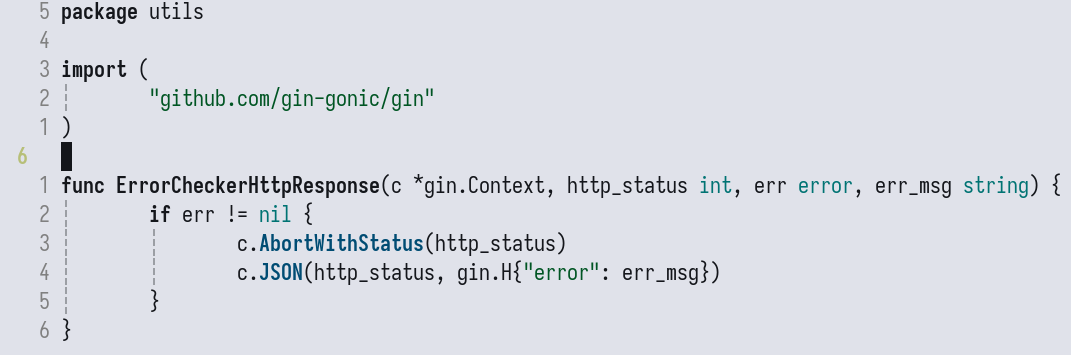
\includegraphics[scale=0.4]{pictures/server_utils.png}
    \caption{Utils layer}
    \label{utilsExample}
\end{figure}

\par
The Models layer contains the structs that represent the entities of the application. 
The structs are used to store the data of the application, and to provide a way to interact with the data.
They also provide a schema of the database, as they are used for mapping the results of the database queries.
Another use for them is to validate the data that is sent to the server, so that we can ensure that the data is correct.

\par
The Database Operations layer contains the functions that interact with the database.
They perform CRUD operations on the database, and to provide the necessary data to the application.
It is the layer that is responsible for the communication between the server and the database.
It's only functionality is the one mentioned above. Other logic, such as validation or error handling, is done elsewhere.
An advantage of writing this layer, instead of choosing and ORM (Object Relational Mapping) library, is that we have more control over the queries that are sent to the database.
This makes the server feel more responsive.

\begin{figure}[htbp]
    \centering
    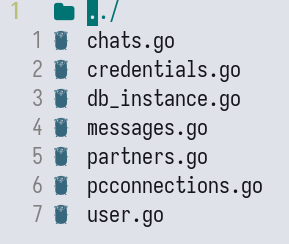
\includegraphics[scale=0.8]{pictures/dboperations.png}
    \caption{Database Operations layer}
    \label{dbOpsExample}
\end{figure}

\par
The Middleware layer goes between the Controllers and the endpoints calls.
It handles the logic that is common to all the endpoints, such as authentication, logging, and error handling.
This makes it easier to add new endpoints, as we don't have to write the same logic for each endpoint.
Also, the handlers for the endpoints can be easily replaced or removed, as they are not tied to the endpoints themselves.

\begin{figure}[htbp]
    \centering
    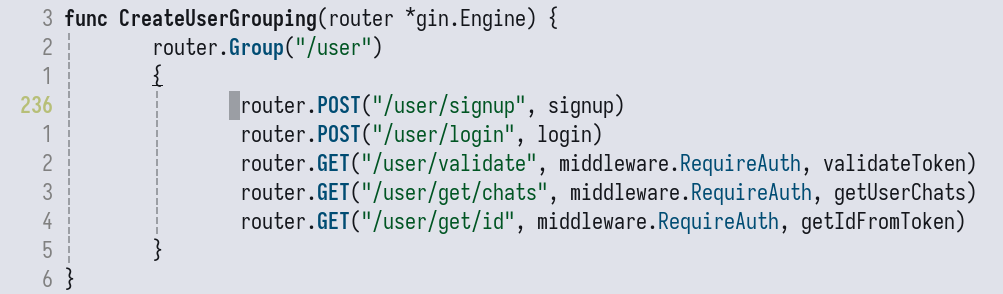
\includegraphics[scale=0.4]{pictures/middleware.png}
    \caption{Middleware layer}
    \label{middlewareExample}
\end{figure}

\par
The Controllers layer contains the functions that handle the requests from the client.
They are used to provide the necessary data to the client, and to handle the data that is sent to the server.
It is the main layer of the server, as they are the ones that interact with the client.
A key point of this layer is that it is not tied to the database, as it only interacts with the Database Operations layer.
I also chose to implement the controllers in a model-based way, as it makes the code more readable and maintainable.

\begin{figure}[htbp]
    \centering
    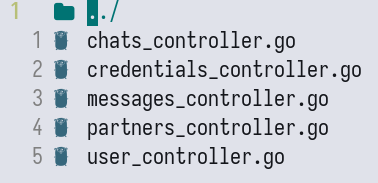
\includegraphics[scale=1.2]{pictures/controllers.png}
    \caption{Controllers layer}
    \label{controllersExample}
\end{figure}

\section{Main focus}
The main entity around which the application is built is the \textit{Partner} class, as seen below.

\begin{figure}[htbp]
    \centering
    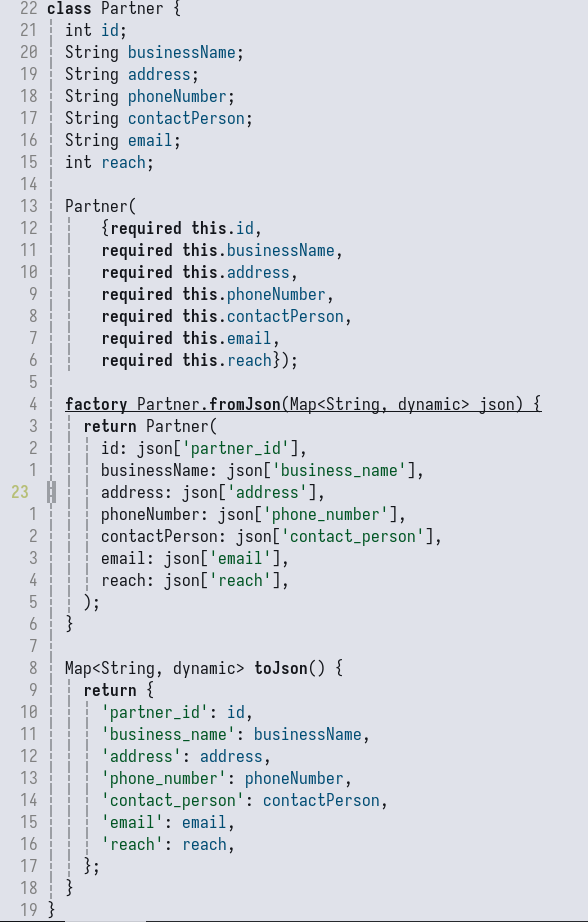
\includegraphics[scale=0.4]{pictures/partner_class.png}
    \caption{Main entity of the application}
    \label{partnersClass}
\end{figure}

This entity is a substitute for the User class, as the User is just a Partner connected with a Credential entity from the DB.
Partner is also connected to the entity Chat, which by itself is connected to Message.
This enforces a good separation of the functionality, and also allows for efficient queries and server responses.
Although this is the main entity, the way it is build, with the additional methods of \textit{fromJson} and \textit{toJson}, allows for easy extension of the application.
This will be present across all the other entities, to manage more easily the bodies of the sent requests.

\par
Now, we'll take a look at how a few components are built, and how their state is managed.
This will contain some good and bad examples, and see how they impact the development of the application, and also the developer experience.

\section{Example Components}
\subsection{Good example}
The first component we'll take a look at is a \textit{Partner list} component. 
To be more specific, the below picture is part of the component that renders the top five partners by reach, a field which represents the average number of clientele.

\begin{figure}[htbp]
    \centering
    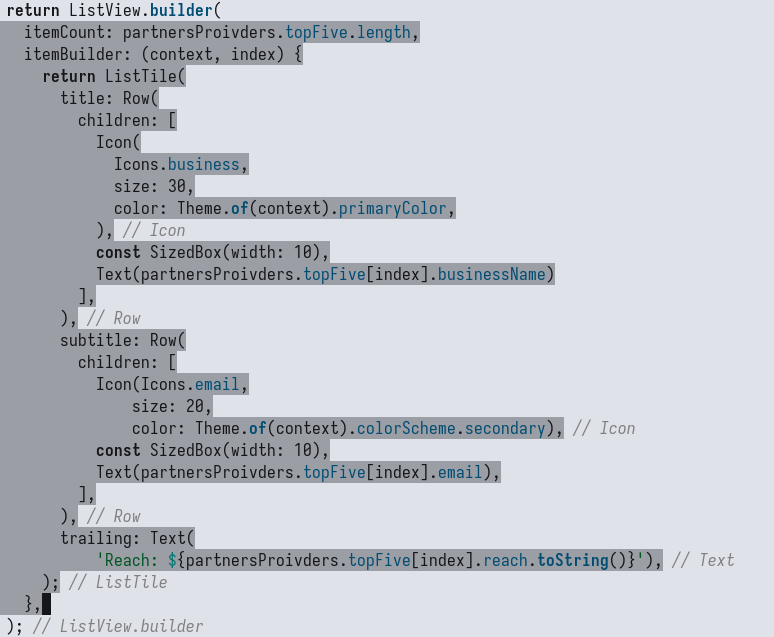
\includegraphics[scale=0.4]{pictures/partners_mapped_good_example.png}
    \caption{List component}
    \label{partnerListComponent}
\end{figure}

Here we can note the good use of states, as the component is stateless, and the state is managed by the provider component.
This is a good practice, as it allows for a more efficient rendering of the component, and also for a more readable code.
Each child sits under a \textit{Consumer} widget, which listens for changes in the provider, and rebuilds the child when the state changes.
By doing so, the component is more efficient, as only the child that needs to be rebuilt is rebuilt, and not the whole component.
Also, it removes for the need of passing the state as a parameter to the child.
Due to the simple nature of the entity is overwatches, it eliminates the need for a websocket.
This is a good example of how to build a component, and how to manage the state of the component, for simple operations on simple entities.

\newpage
\subsection{Bad example}
The second component we'll take a look at is a \textit{Login} component.
This component is used to log in the user, and to provide the necessary data to the application.
In the picture below, we can see that the component is stateful, through the use of controllers.
This is a bad practice, as it makes the component easy to read, but prone to mistakes, due to repetitve coding.

\begin{figure}[htbp]
    \centering
    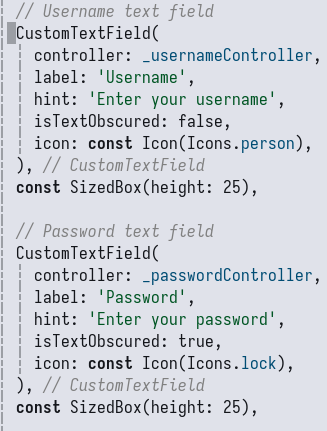
\includegraphics[scale=0.4]{pictures/looks_bad_but_is_good_because.png}
    \caption{Login component}
    \label{loginComponent}
\end{figure}


This is as much avoided as possible, through the makings of custom widgets, that eliminate boilerplate as much as possible.
It is easily observable in the picture below, where \textit{CustomTextField} is used to create a text field, with a custom design, and a custom controller.
Everything under the \textit{Widget build} method would be repeated for each text field, and would make the code harder to read and maintain.
\begin{figure}[htbp]
    \centering
    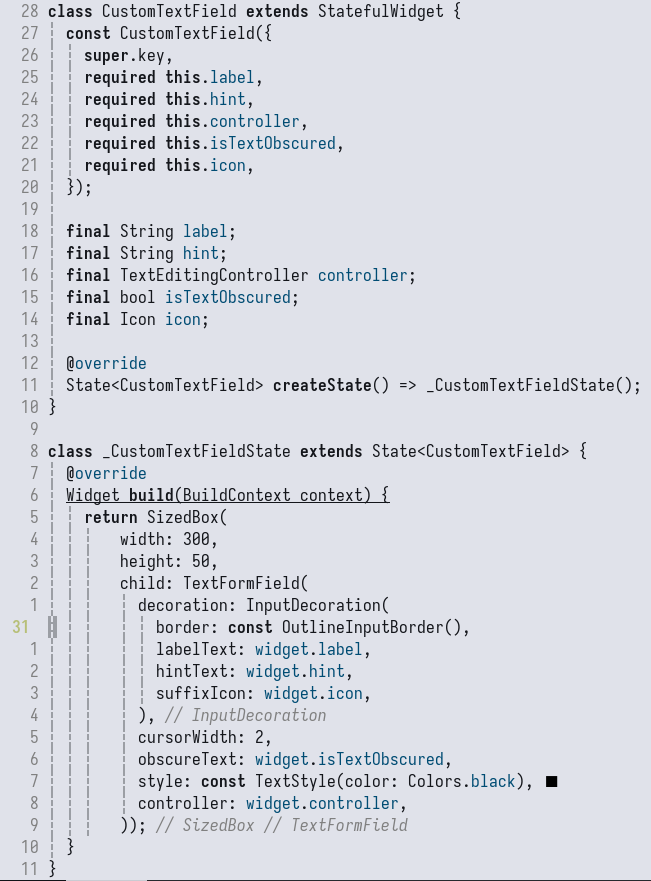
\includegraphics[scale=0.2]{pictures/it_avoid_boilerplate.png}
    \caption{Custom text field}
    \label{customTextField}
\end{figure}



\newpage
\subsection{Neutral example}
The last component we'll take a look at is a \textit{User Details} component.
This component is used to display the details of a user, such as the name, email, and phone number.
It also allows the user to edit the details, and to save the changes.
In the picture below, we can see that the component is stateless, and the state is managed by the \textit{Partners Provider}.

\begin{figure}[htbp]
    \centering
    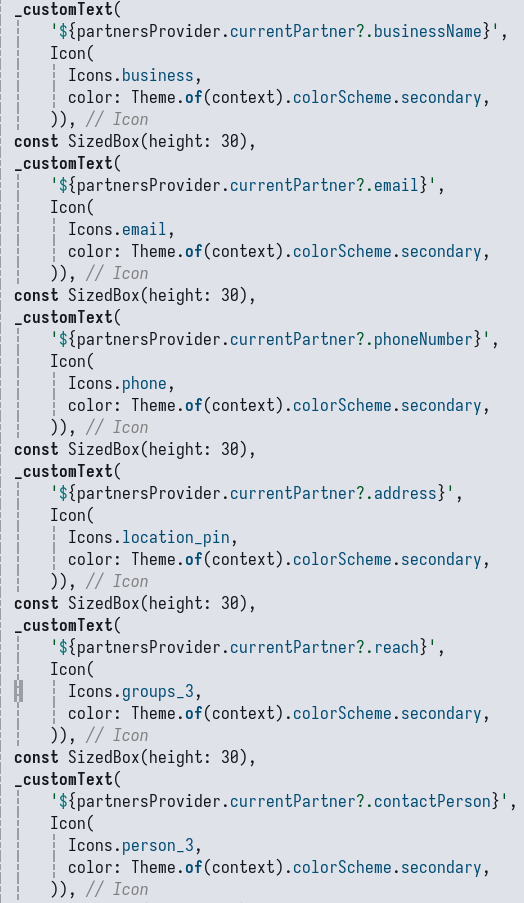
\includegraphics[scale=0.4]{pictures/partners_not_mapped_bad_example.png}
    \caption{User Details component}
    \label{userDetailsComponent}
\end{figure}

This is a bad practice, as it makes the component harder to read, and harder to maintain.
Also, it makes the component less efficient, as there is no need for the whole component to be rebuilt when the provider notifies for changes.
This example, although it is a simple one, shows how not to build a component, and how not to manage the state of the component.
This represents a tricky example, because it looks like a bad mapping, because it is done manually.
In reality, it provides a way to improve the design of the application, by giving custom icons to the inner components.
We can notice this in the picture below.

\begin{figure}[htbp]
    \centering
    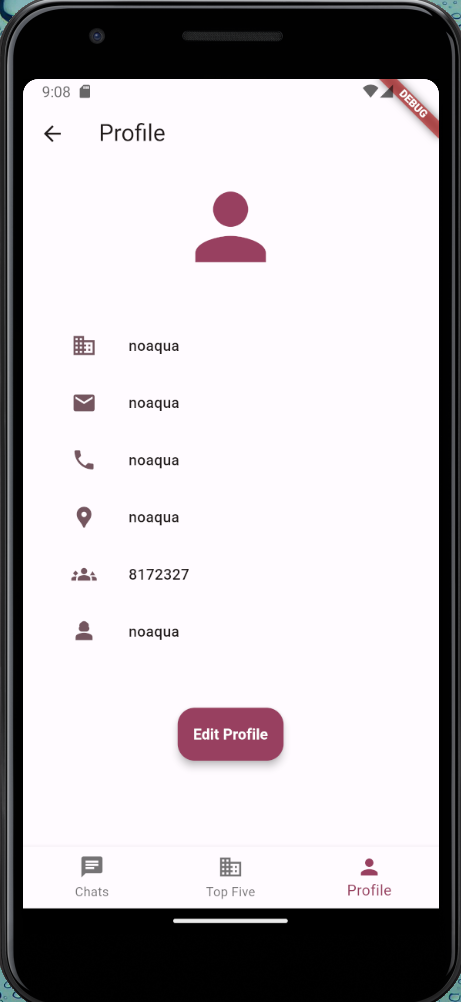
\includegraphics[scale=0.4]{pictures/because_it_looks_bad_we_have_ui.png}
    \caption{User Details UI}
    \label{userDetailsUI}
\end{figure}

\label{implementation}


\chapter{Conclusions}

The research has shown that the use of a cross-platform framework can be beneficial for companies that want to develop applications for multiple platforms.
It can reduce the development time, as the code can be shared between the platforms.
This can also reduce the costs of development, as the developers don't have to learn multiple languages and frameworks.
The research has also shown that the use of a self-implemented server can be beneficial for companies that want to have more control over their data.
It can provide a more realistic scenario, where the data is stored in a company's database, rather than in a third party service.

\par
As noticed in the examples above, the server is separated into different layers, each with its own responsibilities.
The frontend is also separated into different layers, but it requires some manual tweaking in certain use cases.
Both have proven that this separation of concerns can make the code more readable and maintainable, through good and bad examples.
This separation of concerns can also make it easier to add new features to the application, as the code is more organized.

\par
Through the practical implementation of the application, I have learned that the use of a cross-platform framework can be beneficial for companies that want to develop applications for multiple platforms.
Not only that, but the reduction in code duplication can also reduce the development time and costs.
By making use of thoughtful separation of concerns, the code can be more readable and maintainable, and it can be easier to add new features to the application.

\par
It is important to note that the research has some limitations.
The application is developed for Android and Linux devices only, and it uses a self-implemented server.
This means that the application is not available for iOS devices, and it does not use a third party service such as Firebase.
This can limit the reach of the application, as it is not available for all devices.
It can also limit the scalability of the application, as the server is not as robust as a third party service.
But even with these limitations considered, we can still see the benefits of using a cross-platform framework and a self-implemented server, with separation of concerns.


\label{conclusions}

%\addcontentsline{toc}{chapter}{Concluzii}
%\addcontentsline{toc}{chapter}{Conclusions}

\bibliography{references}

\end{document}
%\documentclass[12pt]{scrreprt}
\documentclass[12pt]{report} 

% language may be romanian or english (default is english)
% type may be bachelor or master (default is bachelor)
\usepackage[language=english, type=bachelor]{style}

%\geometry{a4paper,top=2.5cm,left=3cm,right=2.5cm,bottom=2.5cm}
%in style
%controlling the appearance of your headers and footers
\usepackage{fancyhdr}
\pagestyle{fancy}
\lhead{}
\chead{}
\renewcommand{\headrulewidth}{0.2pt}
\renewcommand{\footrulewidth}{0.2pt}

\begin{document}

\specialization{Computer Science}	
\title{Separation of concerns in cross-platform development}					   
\author{Guceanu George - Marian}											
\supervisor{Lect. Dr. Cojocar Dan}				
				
\maketitle


\newpage
\thispagestyle{empty}
\mbox{}
\newpage
\pagenumbering{roman} 

\cleardoublepage


\par
The goal of this thesis is to make an overview of cross-platform development. 
What is the current state of this software development branch, and more importantly what are the main approaches regarding it.
\par
The relevance of this subject is marked by the evergrowing technological advancements. In the past decade more and more machines and platforms came to life that needed to be interoperable and had to communicate with each other. This became a necessity especially because all of them brought alongside different operating systems.
\par 
As a consequence, a lot of development platforms were created. With the increasing relevance for them, more transpositions of the application were needed. It was inconvenient to use an application that is available for only one platform. For the software engineers it meant more code bases that needed maintenance and also a lot more learning.
\par
I will analyze the evolution of software development, what it meant along the decades, from the earliest days, up to the starting point of cross-platform development. This is needed, so we can see the buildup that has been created, turning it into a must-have, rather than a concept. Further on, I'll make a case for the current state of cross-platform development. What are the main features it provides, the legacies it kept from it's predecessors, how it is used today and what are the most important tools used. Then, an analysis over the principle of separating concerns will provide us with the most appreciated features, and see how they align with the needs identified earlier. I will do a breakdown of this principle, see how it has been approached already and why it is a global standard. Afterwards, I will make some regards towards the impact this principle provides, by overlooking some metrics that should provide empirical data, according to the provided examples.

\vspace{0.5cm}	
\hrule
\vspace{0.5cm}	
%\cleardoublepage



\tableofcontents


\newpage
\pagenumbering{arabic}

\chapter{Introduction}

%\chapter*{Introducere}
\label{intro}


Cross-platform development is a modern approach to transitive applications.
It is a domain that gained popularity along the years, due to constant innovations in the gadget realm, such as the smartphone, the tablet or the game console.
Each of these took a different approach on their system design or their operating system, hence creating a multitude of "platforms", all with unique features and perspectives regarding development.
\par
This thesis will have \textit{n} main chapters.
In the first one, we will take a look at the history of development as a whole, and see the turns it took along the years.
In this chapter I will also analyze the evolution of computers, from the earliest times until present.
Then I will link this evolution to software development, to see why cross-platform development turned from a very specific niche to an actual problem.
\par
In the second chapter, I will analyze the current state of cross-platform development.
The first subject will cover the lack of separating concerns in this branch.
I will analyze statistics and observe the consistency that has been preserved throughout the years.
Then, the second subject will be what this branch kept as legacy from its parent derivatives.
To be more exact, this will also be divided into three areas of concern: what are the positive features that live on, regarding several aspects such as performance and code maintenance, what are the negative features that continued out of pure legacy and comfort, and also the features that lie in between the ones aforementioned.
\par
Third chapter will contain an overview and a history of separating concerns as a development principle, and also from an architectural point of view.
This will be a thorough analysis over the positive and negative outcomes that separation of concerns can have.
Then I will make a point by point cover over the advantages this principle proposes and see how it aligns with the upgrades that this branch needs.
\par
In the fourth chapter I will go into more details about the separation of concerns principle.
There will be an in-depth approach towards how it is also separated into different notions, layers and practices.
I will then take the already in-use principles of cross-platform development and separate them, so that they will be fitting the aforementioned layers.
\par
Fifth chapter will cover the impacts of separating concerns.
Here I will do a thorough analysis on the theoretical advantages and disadvantages, and then proceed to measure them.
Collected data will sum up to a report that should prove the above points, all within a given metric.
I will analyze code maintainability, reusability, scalability and more, and see the time complexities, measure memory usage, and then present the challenges regarding debugging, tooling and the learning curve.

%\addcontentsline{toc}{chapter}{Introducere}
%\addcontentsline{toc}{chapter}{Introduction}

\chapter{History of cross-platform development}
\label{chap:ch1}

\indent
\par



%\begin{figure}[htbp]
	%\centering
	%	\includegraphics[scale=0.65]{./figures/fig_3_1.eps}
	%\caption{Ciclul de dezvoltare al sistemelor bazate pe componente adaptat modelului cascadã}
	%\label{FigCBSD}
%\end{figure}
In this chapter, I will elaborate on the progresses made throughout the decades regarding designing software and the evolution of hardware, and see how we ended up with cross-platform development as a necessity.

\section{The 1940-1970 timeline}

\subsection{The 1940's}

\par

During this decade, the "Big Bang" happened.
John Mauchly and Presper Eckert, designed and built the "first digital, electronic computer"\cite{eniacHistory} and came up with the legendary ENIAC.
A computer that was designed with a military goal in mind.
ENIAC was developed at the University of Pennsylvania, being funded by the U.S.
Army, mainly because the teams at the other Universities were not able to keep up with the Army's needs for computing artillery firing tables "for the war 
effort".\cite{eniacDesign}

\par
This computer revolutionized computations as it was the first machine to ever allow any kind of stored procedures, by introducing plugboard wiring and portable function tables in favor of the previous punch cards.
Plugboards were connecting switches, which were "capable of storing one complex instruction for the use of the accumulator".\cite{eniacSwitches}
This meant that, the entirety of the computation was digital, and reconfigurable.
Unfortunately, it also meant that, between each run or change, the computer had to be shut down so the wiring could be redone.
\begin{figure}[htbp]
    \centering
    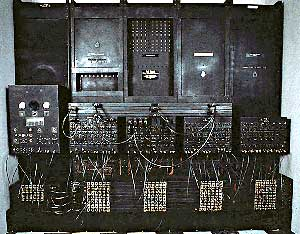
\includegraphics[scale=0.5]{pictures/ENIAC_plugboard_switches.jpg}
    \caption{ENIAC plugboards and switches}
    \label{eniacPlugboardSwitches}
\end{figure}
\par
But, even so, a good algorithm structure was needed, that being mainly because 'these architectural differences lead to some differences in the approach needed for programming'\cite{eniacDesign}.
So the operators of the machine came upon some design and operation principles, that are still observable in the modern world, such as 'Dataflow', 'Parallelism' and 'Looping and branching' \cite{eniacDesign}


\subsection{The 1950's}
\par
Software engineering and designing became a subject of discussion as early as the 1950's.
During those days, this terminology meant something entirely different than what we know of today.
The quote that depicted it quite accurate is: `\textit{Software engineering is like hardware engineering}`\cite{boehmb06}.
This is mainly because software was regarded as building a machine: you embody a plan, manually check it and then get it running on the computer.
\par
The biggest invention of this decade was the concept of storing, organizing and manipulating data.
It is during these times that it got a name, "data processing"\cite{firstDBMS}.
It is also now when the storage, retrieval, and updating of data has been a "key requirement for most computer applications"\cite{firstDBMS}.
These are things that followed up and evolved into the modern world, and they can be observable as most up-to-date applications require enormous data volumes.
Data started to play an important role.
It was regarded as one of the building blocks of applications back then.
This is also another pattern that is kept into the modern development world.
\par
In this same decade, more specifically in 1952, the first compiler was made, for the A-0 system.
This compiler was introduced and put into practice by one of the founding figures of the programming field, that being Grace Hopper.
This represented a turning point, as she proved that computers should understand "human-like" languages\cite{a0compiler}, not the other way around.
Now the tool of software became a much more teachable subject, and had the potential of turning to be more at-hand for everybody.
In 1953 she developed A-2, which is considered to be the first open-source piece of software ever.
That is due to the fact that its source code was given to the customers and they were encouraged to send in possible improvements.


\par
The first commercially-available compiler was put on the market not that later on.
It is the FORTRAN, "formula translator"\cite{a0compiler}, compiler that was developed by IBM in 1957, for the 704 computer.
It is now that we can see a mould for software.
During the same decade, the first pieces of both open-source and closed-source software were developed and put on the market.



\subsection{The 1960's}
During this time period, the machines got a bit more user friendly and code became easily replaceable.
This turned software into something far different to hardware.
COBOL is now introduced to the market, and it made a case for itself.
It is the first programming language that was considered easy to use and read, and that introduced the concept of machine abstraction.
This meant that it did not require a dedicated machine to run.
It was, in a very abstract and distant way, the first piece of cross-platform software.

\par
Now, the ability to rewrite code enabled developers to turn towards a "code and fix" approach\cite{boehmb06}.
This meant that coding was something that did not require as much manual calculations, and that can be thought of and corrected along the way.
Not only that, but it is the first time during this decade that a problem was eradicated: having exact hardware in order to collaborate on development.
This is considered to be a menial job for the modern programmers, but during those times it was a long due issue.
\par
This is one of the biggest turning points in software design, as it allowed for a practice that is still put to good use today.
Correction of code, be it from a logical or opinionated point of view, during development lead to branching and forking, tools that are still used in modern development.



\section{The 1970 - 1990 timeline}
\subsection{The 1970's}
This decade is perhaps the most important step in software development.
This is the decade that made modern computing the thing that we know and love.
In 1972, Dennis M.
Ritchie and his team created the C programming language.
To say it was revolutionary, was an understatement.
This project turned Dennis Ritchie into a titan and unforgettable figure of the software world.
He was a "bearded, somewhat disheveled computer scientist"\cite{ritchieJobs} that stays at the foundation of the things we make most use of today, for exmaple the internet.

\begin{figure}[htbp]
    \centering
    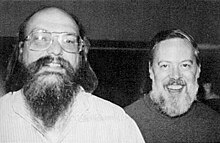
\includegraphics[scale=0.7]{pictures/KenThompson_and_DennisRitchie1973.jpg}
    \caption{Ken Thompson and Dennis Ritchie, 1973}
    \label{unixMakers}
\end{figure}

\par
C is a language that derived from BCPL (Basic Combined Programming Language).
It became relevant when, yet again, Dennis Ritchie decided to use it in order to re-write the source code of the UNIX operating system.
Such and operation was deemed necessary by him mainly because the U.S government categorized the capitalism of such a product as a violation the "Sherman Antitrust Act"\cite{unixRepo}.
Due to this, AT\&T released the Operating System as royalty-free, but later however licenses became a bigger obstruction, hence the limitations in the access of the source code.
Then Dennis Ritchie decided to re-write the whole OS in the high-level programming language in C, in 1973.
This project, although later forked into many other operating systems such MacOS or GNU/Linux, was maintained and developed up to this day to the FreeBSD project.
A part of the legacy assembly source code of UNIX is still on GitHub, at the repository 'dspinellis/unix-history-make'.

\begin{figure}[htbp]
    \centering
    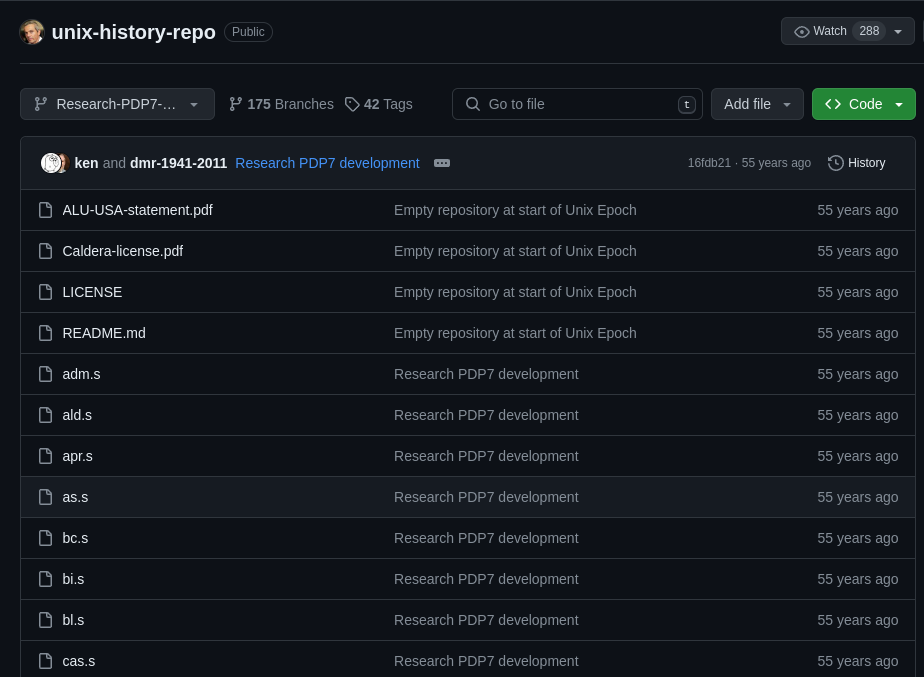
\includegraphics[scale=0.5]{pictures/unix_repo.png}
    \caption{TODO:change to white theme Repository containing the assembly source code of UNIX}
    \label{unixRepo}
\end{figure}


\subsection{The 1980's}
During the 80's, software design became an area on interest for most people involved in the computer science field.
One of the earliest approaches of software design is the Layered architecture.
This was firstly introduced as a need because of the way computer networks were operating.
Now, files were getting bigger and because of that, "The programmer must maintain descriptions of
how various alternative designs are distributed among files"\cite{layeredArchitecure80s}.

\par
Along with these software design paradigms, this decade introduced the first implementation of a version control system.
It worked quite similarly to the modern approaches.
It stored the differentials of the files in a 'delta' file\cite{layeredArchitecure80s}.
This file was one of the deterministic factors for which version control and layered architecture were introduced.
As files grew bigger in size, the delta file associated with it was also getting clunkier, thus making reverting or alternating changes a time and memory-consuming task, and by separating the files into smaller ones, each depending on the other one, this process would be optimized.

\par
This decade brings the most enhancing and used tool of the modern world, the internet.
Although it is believed that invented rather earlier, in the late 60's, it is in 1983 when ARPANET and DDN (Defense Data Network) switched to the TCP/IP standard, "so that computers of many kinds could communicate with each other, no matter what kind of network they were connected to in the Internet".\cite{arpanetDdn} This was a big leap, as ARPANET was an already enormous cluster of interconnected computers, therefore the computers entering the network would have access to them.

\begin{figure}[htbp]
    \centering
    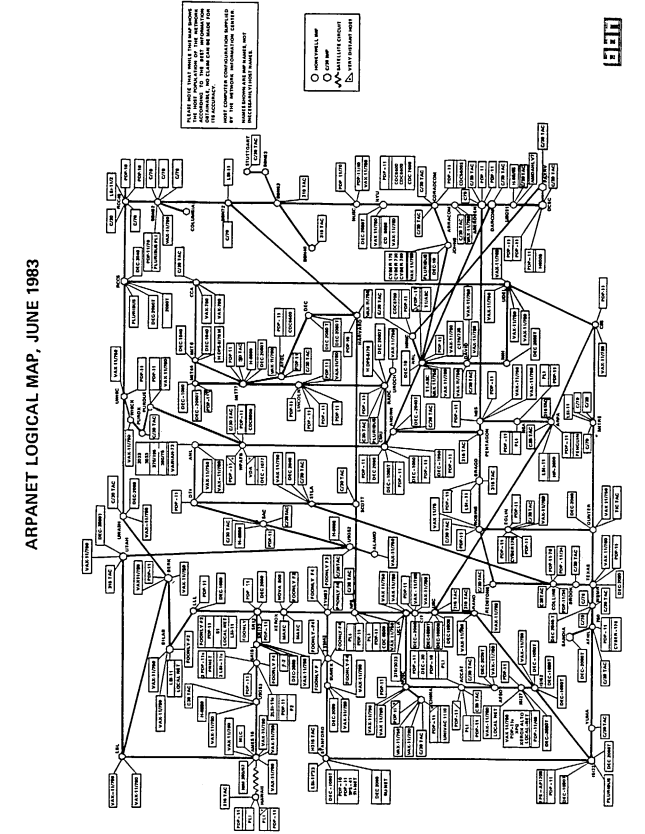
\includegraphics[angle=270,scale=0.35]{pictures/arpanet.png}
    \caption{ARPANET logical map, 1983}
    \label{arpanetLogicaMap}
\end{figure}


\par
Due to this, a doubling of household computers happened until the 90's.
This meant that more people were put on the network, and, due to this, all the computer owners had access to each other's data and information, should they wanted to access it.

\begin{center}
    \begin{tabular}{|| c | c ||}
          \hline
          \textbf{Year} & \textbf{Percentage} \\
          \hline
          1980 & 2.8\% \\
          \hline
          1982 & 6.2\% \\
          \hline
          1983 & 7.3\% \\
          \hline
          1984 & 8.4\% \\
          \hline
          1986 & 9.5\% \\
          \hline
          1988 & 12.5\% \\
          \hline
          1989 & 15.0\% \\
          \hline
    \end{tabular}
\end{center}

\par
As you can see, the biggest jump in the percentages happened between 1980 and 1982.
But, since ARPANET switched their protocols in 1983, the number of computers in personal households has grown by a staggering 7.7\%, a bit more than double.



\subsection{The 1990's}
This decade has been the most influential one for the modern world, and especially for the computing area.
With the evergrowing increase in computer-owning households and the creation of the internet, we see how this affected the development process, thus leading to a series of projects that are major key-factors in our current timeline.

\par
In 1990, we see the first true creation of cross-platform software.
At CERN, Switzerland, Tim Berners-Lee submits two ideas for what should be the Web, back in March 1989.
Until the Christmas of 1990, he contoured the World Wide Web, making the first prototype for it.
The intention of this project was to be "a pool of human knowledge", thus allowing for ease of communication between people who were geologically disjointed\cite{worldWideWeb}.

\par
This project offered features that are still generally available today, such as a server, HTML, the first web programming language, URL's and the first browser.

\section{The 2000's}
\subsection{First definition}
Now, during this decade we can see some of the first mentions of the term "cross-platform development".
That is due to the fact that more and more "platforms" (example: Windows, MacOS) started rising and gaining popularity, and certain large applications needed to behave and act accordingly on all of them.
I will refer to "platform" from now on as development environments, for example Android meaning not only the mobile phone operating system, but also the ecosystem surrounding it, such as smartwatches or TV's.


\par
Some of the first people that proposed this terminology were Bishop J.
and Horspool N., who also gave the first definition to this development branch.
They described the product of it as "software that exists in different versions so that it is available on more than one platform"\cite{firstDefinition}, all the way back in 2006.
In this definition, their meaning of platform is the same as the one I mentioned earlier, because back then the definition was a bit more general, such as "language, operating system, computer, or some combination".
In the same time-period, the Web was starting a world-conquering journey.
Along with it, it brought a whole toolkit of development principles and design patterns, with component-based development being the most praised one.
This is also mentioned and observed by the aforementioned authors, whom agree that component-based development  has made a good impact  toward satisfying "both parts of the definition."\cite{firstDefinition}
\subsection{First toolkits}
The idea of cross-platform development was initially brought as a fix for one of the bigger issues developers faced at the time, and that is building graphical user interfaces (GUI's).
This in itself represented a dilemma because for every platform there were dedicated tools and specific programming languages, for example for Windows there was exclusively .NET with the C\# programming language.
This inherently meant that there was no uniform way of developing such GUI's across platforms.
There is also acknowledgement in this, starting with the earliest days.
Due to such history, there came the stigma that cross-platform toolkits are "integral to GUI development"\cite{firstDefinition}.

\par
Because of this, we can also observe the rise in popularity of some toolkits that were not very seriously taken considered before this realization, such as Qt or GTK+.
These are some of the first cross-platform frameworks that are still used today at a production level, and we can see them used in many well-known applications, such as Spotify for Qt, or the GNOME desktop environment for GTK+.
They are trying to achieve different goals, but one thing that they have in common is that both Qt and GTK+ define a collection of widgets that should work as "platform independent"\cite{firstDefinition}.
This then allowed for the developers to apply a "learn once, code everywhere" approach.

\chapter{Separation of concerns}
Now that we got to understand the origins of cross-platform development, I believe it's time for a move that's just as important for the thesis.
During this chapter, I'll take a step towards a different direction.
I'll take a look at the definitions, because there will be multiple, history, use cases, advantages and disadvantages of the principle of separating concerns.
We'll compare and analyze the views regarding this topic, see where it originated (or all the places of its origins), 
check out what caused it to come into existence, and then do a thorough analysis regarding the benefits it provides, and the disadvantages they bring.


\section{Rise in popularity}
The adoption of the principle of separation of concerns gained significant momentum during the late 20th century and continued into the early 21st century.
While it's challenging to pinpoint an exact time period for its increased adoption, 
we can identify key phases when the concept became more widely recognized and discussed:
\par
During the emergence of object-oriented programming (OOP) in the late 1970s and 1980s, the principles of modularity and separation of concerns gained prominence.
Languages like Smalltalk and Simula popularized OOP concepts such as encapsulation, inheritance, and polymorphism, which inherently promote the separation of concerns.
This period laid the groundwork for the widespread adoption of modular design principles.
\par
The 1990s saw a proliferation of publications and discussions on software design principles, design patterns, and best practices.
Influential works such as "Design Patterns: Elements of Reusable Object-Oriented Software" by the Gang of Four (Erich Gamma, Richard Helm, Ralph Johnson, John Vlissides) were published in 1994.
This book cataloged common design patterns, many of which emphasize separation of concerns.
The 1990s also witnessed the rise of agile methodologies and the growing importance of modular design in software development.
\par
In the early 2000s, there was a continued focus on modular design principles, particularly within the context of domain-driven design (DDD) and agile software development.
Eric Evans' book "Domain-Driven Design: Tackling Complexity in the Heart of Software" (2003) emphasized the importance of separating concerns within a software system to improve maintainability and alignment with business requirements.
This period saw an increasing recognition of separation of concerns as a fundamental principle in software architecture.
\par 
From the mid-2000s to the present day, separation of concerns has remained a central tenet of software engineering practices.
The advent of microservices architectures, cloud computing, and DevOps practices further underscored the importance of modular design and loose coupling.
Additionally, the proliferation of open-source software projects and collaboration platforms facilitated the exchange of knowledge and best practices related to separation of concerns.
\par
Overall, while separation of concerns has been a guiding principle in software engineering for several decades, its adoption 
and recognition as a fundamental design principle gained momentum during the late 20th century and continue to shape software development practices today.
The most significant publications about separation of concerns were written during the 1990s and early 2000s, 
coinciding with the emergence of object-oriented programming and the proliferation of design patterns and agile methodologies.


\section{Definition}
Separation of concerns is a design principle in software engineering where different parts of a system are divided to handle different responsibilities.
This makes the system easier to understand, maintain, and modify because each part focuses on a specific aspect of functionality, 
rather than trying to handle everything at once.
It is a fundamental principle in software architecture that promotes modularity, maintainability, and scalability, or, as Harold Ossher and Peri Tarr put it, 
it's something that stands at the "core of software engineering" \cite{definitionSOC}.
\begin{figure}[htbp]
    \centering
    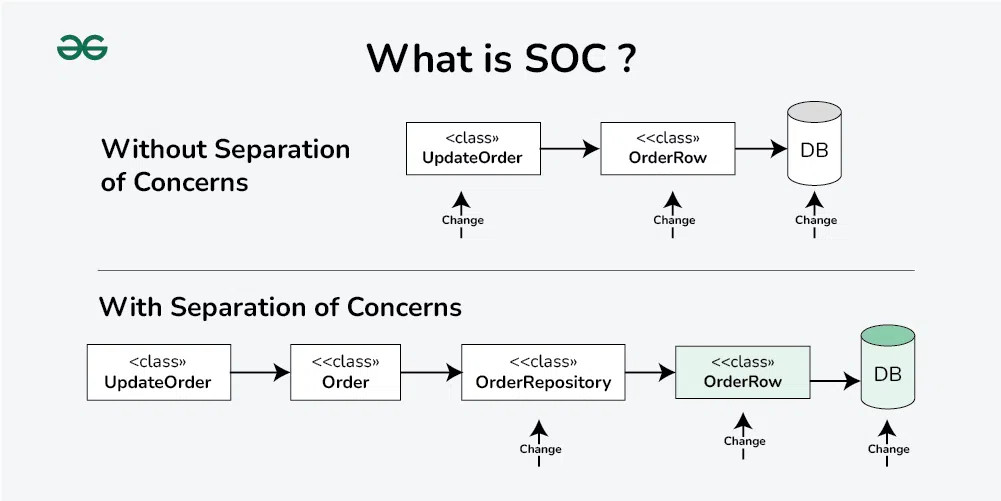
\includegraphics[scale=0.4]{pictures/soc_definition_example.jpg}
    \caption{Separation of concerns definition example, source: \href{https://www.geeksforgeeks.org/separation-of-concerns-soc/}{GeekForGeeks}}
    \label{arpanetLogicaMap}
\end{figure}
\par
Now we'll take an in-depth look at the founding ideas that are holding this principle high in its regard.
These are: modularity, flexibility and reusability, testing and scalability.
We'll take each of them apart and see what they can provide for us.


\subsection{Modularity}
Separation of concerns promotes modularity, where a system is divided into smaller, independent modules.
Each module encapsulates a specific aspect of functionality.
For example, in an application that requires extensive security, 
advanced separation of concerns allows for building mechanisms that "can be merged into the system in a flexible way" \cite{socExample}.
\par
Modularity encourages encapsulation, which involves bundling related functionality and data into cohesive units called modules.
Each module represents a self-contained unit of code that hides its internal implementation details from the rest of the system.
This encapsulation fosters information hiding, reducing dependencies between modules and promoting loose coupling.
\par
Modular design emphasizes defining clear and well-defined interfaces for communication between modules.
These interfaces specify how modules interact with each other, providing a contract that ensures consistent behavior and interoperability.
By adhering to these interfaces, developers can swap out implementations or extend functionality without affecting other parts of the system, as long as the interface remains unchanged.
\par
Modularity allows for varying levels of granularity in module design.
Modules can be large or small, depending on the complexity and scope of the functionality they encapsulate.
Decomposing a system into smaller, more manageable modules facilitates better organization and promotes code reuse.
However, it's essential to strike a balance between granularity and cohesion to avoid overly fragmented or tightly coupled modules.
\par
Overall, modularity is a key aspect of the separation of concerns principle that promotes the organization, maintainability, and extensibility of software systems.
By breaking down a system into modular components with clear interfaces and well-defined responsibilities, developers can create more flexible, scalable, and reusable codebases.


\subsection{Readability and Maintainability}
By separating concerns, the code becomes easier to read and understand.
This is important, becuase it was proven by Raymond P. L. Buse and Westley R. Weimer that 
"low readability correlates more strongly with this direct notion of defect density" \cite{readabilityMaintainability}.
Developers can focus on one aspect of the system at a time, making it easier to debug, maintain, and modify without affecting other parts of the system.
This also facilitates collaboration among team members, as each person can work on different modules independently.
\par
Separation of concerns promotes clear code organization by dividing a system into distinct modules, each responsible for a specific aspect of functionality.
This modular structure makes it easier for developers to locate and understand relevant code when working on a particular feature or fixing a bug.
Clear organization reduces cognitive overload and helps developers navigate the codebase more efficiently, improving readability.
\par
By isolating concerns into separate modules, separation of concerns reduces the complexity of individual components.
Each module focuses on a specific task or responsibility, which makes the code more concise and easier to comprehend.
Developers can reason about each module in isolation, without having to consider the entire system's complexity at once, leading to improved readability.
\par
Separation of concerns aligns with the Single Responsibility Principle (SRP), which states that a module or class should have only one reason to change.
By adhering to SRP, modules become more focused and maintainable, as they are less likely to be affected by changes unrelated to their primary responsibility.
This principle enhances readability by promoting a clear understanding of each module's purpose and minimizing code churn during maintenance.
\par
Separation of concerns facilitates modular testing, where each module can be tested independently of the rest of the system.
This modular approach to testing improves maintainability by allowing developers to identify and fix bugs more efficiently.
Unit tests can be written for each module to verify its behavior in isolation, making it easier to pinpoint and resolve issues without disrupting other components.
\par
To sum it up, separation of concerns enhances readability and maintainability by promoting clear code organization, reducing complexity, adhering to the Single Responsibility Principle, isolating changes, facilitating modular testing, and encapsulating complexity.
By breaking a system into modular components with well-defined responsibilities, developers can create codebases that are easier to understand, modify, and maintain over time.


\subsection{Flexibility and Reusability} 
Separating concerns allows for greater flexibility and reusability of code.
We need to understand that flexibility is a key aspect of software design, as it allows for adapting to changing requirements and environments.
Through separation of concerns, we can ensure that we have solid base for reusability, because, as Jones T.C. mentioned,
"effective reuse will require an architectural starting point" \cite{flexibilityReusability}.
Since each module is designed to handle a specific responsibility, it can be reused in different parts of the system or even in other projects altogether.
For example, a module responsible for database access can be reused in multiple parts of an application without modification.
\par
Separation of concerns enables a flexible system architecture by allowing each module to focus on a specific aspect of functionality.
This modular approach means that individual modules can be modified, replaced, or extended without affecting other parts of the system.
For example, if you need to change the data storage mechanism in your application, you can modify the database module without altering the modules responsible for business logic or user interface presentation.
\par
Modular design facilitates the creation of plug-and-play components that can be easily integrated into different systems or projects.
By encapsulating functionality within self-contained modules, developers can reuse these components across various applications without modification.
This promotes code reuse, accelerates development, and ensures consistency across projects.
\par
Separation of concerns encourages the creation of a library of reusable modules that can be leveraged across different projects.
These modules encapsulate common functionality, such as authentication, data validation, or file handling, making them readily available for use in new projects.
By building a library of reusable components, developers can reduce development time, minimize duplication of effort, and maintain consistency in software architectures.
\par
Separation of concerns facilitates integration with third-party libraries, frameworks, or services.
By encapsulating integration logic within modular components, developers can easily swap out implementations or upgrade dependencies without affecting the rest of the system.
This interoperability enables software systems to leverage external resources and functionalities, enhancing their capabilities and reducing development effort.
\par
When concerns are separated, changes and updates can be isolated to specific modules without affecting the rest of the system.
This isolation minimizes the risk of unintended consequences and makes it easier to test and validate modifications.
Developers can confidently refactor or extend individual modules knowing that they won't inadvertently impact other parts of the codebase, which enhances maintainability.
\par
Separation of concerns facilitates modular testing, where each module can be tested independently of the rest of the system.
This modular approach to testing improves maintainability by allowing developers to identify and fix bugs more efficiently.
Unit tests can be written for each module to verify its behavior in isolation, making it easier to pinpoint and resolve issues without disrupting other components.
\par
Modular design encapsulates complexity within well-defined boundaries, making the codebase more maintainable.
By hiding implementation details behind module interfaces, developers can interact with modules at a higher level of abstraction, reducing cognitive overhead.
This encapsulation shields developers from unnecessary complexity, enabling them to focus on understanding and maintaining one concern at a time, which enhances readability and maintainability.
\par
In summary, separation of concerns fosters flexibility and reusability by enabling modular, self-contained components that can be easily integrated, customized, extended, and reused across different projects and contexts.
This promotes agility, reduces development time, and facilitates the creation of scalable and adaptable software systems.


\subsection{Testing} 
When concerns are separated, it becomes easier to test individual modules in isolation.
This allows for more targeted and comprehensive testing, as each module can be tested independently of the rest of the system.
Additionally, modular code is often easier to mock or stub, which is useful for unit testing.
Testing is a need that should be more enforced, because "software bugs will almost always exist" \cite{testing}.
\par
Separation of concerns facilitates modular testing, where each module can be tested independently of the rest of the system.
This modular approach allows developers to write focused unit tests for individual modules, verifying their behavior in isolation.
By decoupling modules from their dependencies, such as external services or databases, developers can easily mock or stub these dependencies to create controlled test environments.
\par
When concerns are separated, testing becomes more focused and targeted.
Each module encapsulates a specific aspect of functionality, making it easier to identify and test individual behaviors.
By isolating concerns, developers can write tests that validate the correctness of each module's behavior without having to consider the interactions with other parts of the system.
This isolation simplifies testing and reduces the scope of potential failures, improving test coverage and reliability.
\par
Separation of concerns promotes clear test scenarios by defining well-defined boundaries between modules.
Each module has a clear interface and defined inputs and outputs, making it easier to identify test cases and expected outcomes.
Developers can write tests that cover various scenarios and edge cases for each module, ensuring comprehensive test coverage and robustness.
\par
Modular design enables parallel testing, where multiple modules can be tested concurrently.
Since each module operates independently of the others, developers can run tests for different modules simultaneously, reducing overall test execution time.
This parallel testing approach accelerates the feedback loop and improves the efficiency of the testing process, enabling faster iteration and delivery of software updates.
 \par
Separation of concerns enhances test maintainability by minimizing the impact of changes on test suites.
When concerns are isolated into separate modules, modifications to one module are less likely to affect the tests for other modules.
This decoupling between modules and tests reduces the need for extensive test refactoring when making changes to the codebase, ensuring that tests remain valid and reliable over time.
 \par
While separation of concerns primarily facilitates unit testing, it also supports integration testing by providing clear interfaces between modules.
Integration tests validate the interactions and collaborations between modules to ensure that they work together correctly as a cohesive system.
By testing integration points and boundary conditions, developers can identify and resolve integration issues early in the development lifecycle, improving overall system reliability.


\subsection{Scalability}
Separating concerns also facilitates scalability.
As the system grows and evolves, new functionality can be added. Existing functionality can be modified without affecting other parts of the system.
This makes it easier to scale the system both horizontally (by adding more instances of existing modules) and vertically (by adding new modules).
It also refers to the performance of an existing system, as "performance and scalability are about the scalable performance of the system" \cite{scalability}.
Let's take a more in-depth look at how it influences scalability.
\par
By dividing a system into independent modules, each responsible for a specific concern, it becomes easier to manage and scale individual components.
For example, in a web application, the user interface, business logic, and data storage can be separated into distinct modules.
This isolation allows each part to be scaled independently based on demand.
Modules can be scaled according to their specific load requirements.
For instance, if the data storage module experiences heavy read/write operations, it can be scaled up by adding more database instances or using a distributed database system, without affecting the business logic or user interface modules.
\par
Separation of concerns allows for distributing the load across different modules running on separate servers or instances.
For example, microservices architecture, which heavily relies on SoC, enables distributing microservices across different nodes.
This distribution helps balance the load effectively, preventing any single component from becoming a bottleneck.
Components can be replicated across multiple servers to handle increased traffic.
For instance, multiple instances of a stateless service (e.g., an authentication service) can be run behind a load balancer to handle a larger number of requests concurrently.
\par
By isolating concerns, resources such as CPU, memory, and storage can be allocated more efficiently.
Each module can be optimized for its specific workload.
For example, a caching module can be allocated more memory, while a computation-intensive module can be allocated more CPU resources.
Cloud platforms provide features like auto-scaling, where resources are automatically added or removed based on current demand.
SoC makes it easier to apply elastic scaling to individual components, ensuring that resources are used efficiently and costs are controlled.
\par
Separation of concerns allows for optimizing the performance of individual modules without affecting the entire system.
For example, performance-critical modules such as a real-time analytics engine can be highly optimized for speed and efficiency, while less critical modules can be optimized for maintainability or other factors.
Separation of concerns facilitates the implementation of asynchronous processing.
For example, background tasks like data processing or logging can be handled by separate modules running asynchronously, reducing the load on the main application and improving overall responsiveness.
\par
When concerns are separated, updating or upgrading individual modules becomes simpler.
New features or improvements can be added to specific modules without disrupting the entire system, making it easier to evolve and scale the system over time.
Separation of concerns allows for incremental scalability, where new modules can be added to handle additional concerns as needed.
This approach ensures that the system can grow organically, adapting to new requirements and scaling efficiently.
\par
By isolating concerns, failures in one module are less likely to affect other parts of the system.
For example, if the payment processing module in an e-commerce application fails, it doesn't impact the product catalog or user authentication modules.
This isolation improves the overall resilience and scalability of the system.
In the event of partial system failures, separation of concerns allows for graceful degradation.
Non-critical modules can fail or scale down without taking down the entire system, ensuring that critical services remain operational and scalable.
\par
In summary, separation of concerns enhances scalability by enabling modular architecture, efficient resource allocation, targeted performance optimization, easier maintainability and extensibility, and improved fault isolation and recovery.
By organizing a system into distinct, manageable components, this design principle allows for focused scaling efforts, better resource utilization, and a more resilient and adaptable architecture.


\section{Challenges}
While the benefits of separating concerns are well-documented, the paradigm also introduces several challenges that developers and architects must navigate to realize its full potential.
These challenges span various aspects of software development, including design complexity, increased component management, inter-module communication, dependency management, integration testing, configuration management, and team coordination.
Understanding these challenges is crucial for effectively applying the principle and leveraging its advantages without succumbing to the pitfalls that can arise from increased system complexity.
Now we'll take a look at the mentioned challenges and analyze them.

\subsection{Complexity}
From a design perspective, separating concerns often requires designing a system with multiple modules, each responsible for a specific aspect of the functionality.
This aspect is one of the hardest to quantify, because "the base of every evaluation of the complexity of a program is an idea" \cite{complexity}.
Taken this into consideration, we'll enforce the following definition of complexity:
modular design can be complex because it involves defining clear boundaries and interfaces between modules.
Ensuring that each module interacts correctly and efficiently with others can be challenging, particularly in large systems with many interdependencies.
Deciding how to partition a system into separate concerns can be non-trivial. It requires a deep understanding of the domain, potential changes, and future scalability requirements. Poorly defined boundaries can lead to tight coupling between modules, defeating the purpose of SoC.
\par
As concerns are separated, the number of components in the system increases. Managing these components, keeping track of their versions, and ensuring they are correctly integrated into the overall system can add significant complexity. Each component may have its own lifecycle, dependencies, and configuration requirements.
Deploying a system composed of many separate components can be more complex than deploying a monolithic system. Each component might need to be deployed independently, and the interactions between them must be carefully managed to ensure the system functions correctly as a whole.
\par
When enforcing the principle, different concerns are handled by different modules, which need to communicate effectively. Managing this communication can be complex, especially when different modules are developed by different teams or even at different times. Choosing the right communication protocols and ensuring data consistency across modules are critical challenges.
In a distributed system, maintaining synchronization between different modules can be difficult. Issues like data consistency, latency, and failure handling become more prominent as the number of communicating modules increases.
\par
While it aims to reduce dependencies between modules, some level of interdependency is inevitable. Managing these dependencies and ensuring that changes in one module do not adversely affect others can be complex. Dependency injection and service discovery mechanisms can help but add another layer of complexity to the system.
Keeping track of different versions of modules and ensuring compatibility between them can be challenging. This is particularly true in environments where modules are developed and released independently.
In summary, to address complexity issues, we need to keep in mind an overhead of design and architectural challenges, managing an increased number of components, ensuring effective communication and synchronization between modules, handling dependencies and versioning, and managing configurations. Addressing these challenges requires careful planning, robust tooling, and effective communication among development teams.

\subsection{Performance}
When a system is divided into separate modules, these modules often need to communicate with each other. This communication, whether it’s through function calls, message passing, or network requests, introduces latency. For instance, in a microservices architecture, each service call over the network adds a delay, which can accumulate and degrade overall system performance.
Data exchanged between modules often needs to be serialized and deserialized, especially in distributed systems. This process can be computationally expensive and add to the latency, particularly when dealing with large volumes of data or complex data structures.
\par
In systems where concurrency is heavily used, such as those employing multiple threads or asynchronous processing, the operating system may need to perform frequent context switches. This switching incurs overhead, as the CPU must save and restore the state of threads or processes, potentially leading to reduced performance.
Separate modules may require their own resources, such as memory and CPU cycles. Inefficient use of these resources across modules can lead to increased computational overhead. For example, if each module maintains its own data cache, it can lead to duplicated data and higher memory usage.
\par
In distributed systems where modules communicate over a network, the amount of data transferred between modules can become significant. High network traffic can saturate the network bandwidth, reducing throughput and affecting the performance of other network-dependent operations.
If a particular module becomes a communication bottleneck, it can slow down the entire system. For instance, a centralized database or a service handling authentication might become a performance bottleneck if it cannot handle the volume of requests efficiently.
\par
Optimizing the performance of a system with separated concerns requires comprehensive profiling and monitoring across all modules. This can be complex and resource-intensive. Identifying performance bottlenecks necessitates detailed insights into the interactions and performance metrics of each module.
Performance optimization often requires coordinated changes across multiple modules. For instance, optimizing a data processing pipeline might involve adjustments in both the data ingestion module and the processing module. Ensuring that these optimizations are harmonized can be challenging.
\par
In summary, performance challenges  need careful management, and by understanding and addressing these challenges, developers can create systems that leverage the advantages of separating concerns without compromising on performance.

\subsection{Learning curve}
Applying the principle in software development introduces a learning curve that can be challenging for developers, 
particularly those new to the paradigm or working within complex systems. 
Now, let's do an in-depth analysis at the specific learning curve challenges.
\par
Separation of concerns requires developers to think differently about how they design and structure their code. Instead of creating monolithic applications, they must learn to break down functionality into distinct, loosely-coupled modules. This shift in thinking can be difficult, especially for those accustomed to traditional, tightly-coupled designs.
Effective application of the principle demands a solid grasp of software architecture principles, including how to define clear interfaces, manage dependencies, and ensure proper module interactions. Developing these skills takes time and experience.
\par
Setting up a project while keeping the principle in mind involves creating and configuring multiple modules from the outset. This can be more complex and time-consuming than starting with a monolithic approach, requiring a good understanding of project organization and configuration management.
Developers need to familiarize themselves with tools and frameworks that also encourage the use of the principle. For instance, in a microservices architecture, knowledge of containerization (e.g., Docker), orchestration (e.g., Kubernetes), and service discovery tools becomes essential. The learning curve for these technologies can be steep.
\par
The principle often relies on well-established design patterns (e.g., Observer, Strategy, Factory, MVC, the last one being later used in a demonstrated implementation). Developers need to learn these patterns and understand when and how to apply them effectively. This involves both theoretical knowledge and practical experience.
Beyond design patterns, developers must also familiarize themselves with best practices for implementing SoC, such as encapsulation, loose coupling, and high cohesion. These principles are essential for creating maintainable and scalable systems.
\par
In summary, by providing the necessary training, tools, and support, developers overcome these challenges and effectively apply the principle to create maintainable, scalable, and high-performing systems.

\subsection{Tooling}
Implementing the separation of concerns principle in software development often necessitates the use of specialized tools to manage the increased complexity of modular systems. 
While these tools can greatly enhance the development process, they also introduce several challenges. 
Now we'll dive deeper and look at the tooling challenges associated with the principle.
\par
There is a vast array of tools available for different aspects of software development, such as version control, build automation, testing, deployment, and monitoring. 
Selecting the right combination of tools that work well together and support that support the principle can be daunting.
Once chosen, integrating these tools into a cohesive development environment can be challenging. 
Ensuring that the tools communicate effectively, and that workflows are streamlined requires careful planning and configuration. 
Integration issues can lead to inefficiencies and disruptions in the development process.
\par
Setting up the development environment to support separation of concerns typically involves configuring multiple tools and ensuring they are correctly set up for different modules. This setup can be time-consuming and complex, especially for large projects.
Ensuring that all developers have consistent environments can be difficult. Discrepancies in tool versions, configurations, or dependencies can lead to “it works on my machine” issues, where code behaves differently on different setups.
\par
In summary, by selecting the right tools, providing comprehensive training and documentation, automating setup processes, maintaining tools regularly, streamlining debugging, and planning for scalability, organizations can effectively mitigate these challenges and leverage the full benefits of this principle.


\subsection{Debugging}
Applying the separation of concerns principle introduces several debugging challenges due to the modular and often distributed nature of the system. 
Debugging is a step that's quite often met in the development process, because it "typically happens during three activities" \cite{debugging} of this process.
Let's take a look at these challenges.
\par
In a system where concerns are separated into distinct modules or services, identifying the source of an issue can be challenging. A bug in one module might manifest as an error in another, leading to confusion about where the problem actually lies.
Debugging issues that span multiple modules requires understanding the interactions and dependencies between them. This complexity increases with the number of modules and their interconnections.
\par
Each module might have its own logging mechanism, making it difficult to trace the flow of events across the entire system. Consolidating logs from different modules into a centralized logging system is essential but can be complex to set up and maintain.
Maintaining context (such as transaction IDs or user session information) across module boundaries is crucial for effective tracing. Ensuring this context is consistently propagated throughout the system can be challenging.
\par
Reproducing issues in a modular system can be difficult due to differences in development, testing, and production environments. Ensuring consistency across these environments is key but can be resource-intensive.
Each module may manage its own state, making it harder to reproduce issues that depend on specific states across multiple modules. Capturing and restoring these states for debugging purposes adds complexity.
\par
Different modules might have different error handling strategies, leading to inconsistencies in how errors are reported and propagated. Ensuring a unified error handling approach across modules is essential for effective debugging.
Debugging asynchronous operations, such as those involving message queues or background processing, adds another layer of complexity. Tracing the lifecycle of an asynchronous task across modules requires specialized tools and techniques.
\par
In summary, by employing centralized logging, distributed tracing, consistent environments, effective state management, integrated debugging tools, performance considerations, and standardized error handling, developers can mitigate these challenges and enhance their ability to debug complex modular systems effectively.

\label{chap:ch3}

\chapter{Current state of cross-platform development}

\section{Overview}

Cross-platform software is designed to operate on multiple computing platforms, such as different operating systems (Windows, macOS, Linux) or device types (desktop computers, mobile devices, web browsers).
The primary goal of cross-platform development is to write a single codebase that can run on various platforms with minimal modifications, thereby reducing development time and cost while maximizing reach and usability.
Now we will take a look at some key-features of this type of development.

\subsection{Code Reusability}
This development area can be best categorized into two types of codebases: single codebase and shared libraries and frameworks.

\par
Developing with a single codebase means that the same code can be reused across multiple platforms, reducing duplication and making maintenance easier.
Also, due to this approach, the need for dependency checking is eliminated, as it is one of the most daunting tasks regarding cross-platform development.
A good scenario, for example, is to know that your application's server is dependent on an Object-Relational Mapping (ORM) framework, or a wrapper for one to be more specific, and to find that it is being discontinued.
This is where single codebase comes in, as it is not dependent on a framework, a package or a library, but on the code itself, thus making it more reliable and easier to maintain. 
The disadvantage of this approach is that it can be more time-consuming and expensive to develop, as it requires more effort to write and test the code.

\par
Utilizing shared libraries and frameworks, such as .NET Core, Flutter, or JavaScript frameworks (e.g., React Native, Electron), helps streamline development.
These libraries and frameworks provide pre-built components and tools that can be used across multiple platforms, reducing the amount of code that needs to be written and tested.
However, the downside of this approach is that it can be more challenging to maintain and update the codebase, as changes to the library or framework may require modifications to the application code.
In addition, the performance of the application may be affected by the overhead of the library or framework.

\subsection{Platform Abstraction}
Platform abstraction refers to building an abstraction layer that isolates the application logic from the platform-specific code (e.g. Kernel interactions).
It is necessary, due to the multitude of platforms that exist today, each with its own set of features and requirements.

\par
Abstraction layers allow developers to write platform-agnostic code that interfaces with platform-specific functionality through standardized APIs.
They are also one of the core features of separating concerns, as they provide a clear separation between the application logic and the platform-specific code.
This allows developers to focus on writing the core functionality of the application without having to worry about the underlying platform details.
In addition, abstraction layers can help improve code maintainability and portability, as changes to the platform-specific code can be isolated and managed more easily.

\par
Middleware provides a layer between the application and the operating system, handling differences in platform-specific operations.
It can be used to abstract away platform-specific details, such as file system access, network communication, and user interface interactions.
Middleware can also provide additional functionality, such as caching, logging, and error handling, that can be shared across multiple applications.
However, middleware can introduce additional complexity and overhead, as it adds an extra layer of abstraction between the application and the platform.

\subsection{Conditional Compilation and Code}
Conditional compilation is a technique used to include or exclude code based on the target platform or configuration.
This involves writing code that compiles differently depending on the target platform, often using preprocessor directives or build configurations.
Sometimes, platform-specific code is necessary to handle unique features or limitations of each platform.
This is necessary especially on the application's user interface, as each platform has its own design guidelines and user experience expectations.



\section{Legacy paradigms that are present today}
We will take a look at all the features that cross-platform development kept from its predecessors, and see how they align with the needs identified earlier.

\par
Despite the evolution of software development practices, several legacy design principles have remained relevant and continue to be applied in modern cross-platform development. 
These principles provide a foundation for creating robust, maintainable, and scalable applications. 
Here are some key legacy design principles still in use today.

\subsection{Separation of Concerns} 
This sounds confusing now, but the principle is implemented in a very shallow and basic way, as it is not a global standard.
This can be observed in the lower levels of the application, where the concerns are separated into platform-specific and platform-agnostic code.
However, this separation is not always clear or consistent, as platform-specific code may be mixed with platform-agnostic code, leading to dependencies and coupling between different components.
This can make it difficult to maintain and update the codebase, as changes to one component may require modifications to other components as well.
It is also worth mentioning that the principle is not used as intended in the higher levels of the application, where the concerns are mixed together, leading to increased complexity.

\subsection{Single Responsibility Principle (SRP)}
The Single Responsibility Principle (SRP) states that a class should have only one reason to change.
This principle is relevant in cross-platform development, as it helps to create more modular and maintainable code.
By separating concerns into individual classes or components, developers can isolate changes to specific areas of the codebase.
\par
This makes it easier to understand, test, and modify the code, as each component has a clear and well-defined purpose.
However, the SRP is not always followed in cross-platform development, as classes or components may have multiple responsibilities.

\subsection{DRY (Don't Repeat Yourself)}
The DRY principle states that code should not be duplicated, but instead should be reused or abstracted into shared components.
This principle is relevant in cross-platform development, as it helps to reduce redundancy.
By reusing code across multiple platforms, developers can save time and effort, as changes only need to be made in one place.
However, the DRY principle is not always followed in cross-platform development, as code duplication can occur due to platform-specific requirements or limitations.

\subsection{Open/Closed Principle}
The Open/Closed Principle states that classes should be open for extension but closed for modification.
This principle is relevant in cross-platform development, as it helps to create more flexible and maintainable code.
By designing classes to be extensible, developers can add new functionality without modifying existing code.
This makes it easier to adapt the codebase to changing requirements or new platforms.

\subsection{Liskov Substitution Principle}
The Liskov Substitution Principle states that objects of a superclass should be replaceable with objects of a subclass without affecting the correctness of the program.
This principle is relevant in cross-platform development, as it helps to ensure that code is reusable and interoperable across different platforms.
By designing classes to be substitutable, developers can create more flexible and scalable code.
However, the Liskov Substitution Principle is not always followed in cross-platform development, as platform-specific code may not be interchangeable with platform-agnostic code.

\subsection{Dependency Injection (DI)}
Dependency Injection (DI) is a design pattern that allows objects to be injected into a class rather than created internally.
This pattern is relevant in cross-platform development, as it helps to decouple components and reduce dependencies.
By injecting dependencies into classes, developers can create more modular and testable code.
However, DI is not always used in cross-platform development, as it can add complexity and overhead to the codebase.

\subsection{Lack of separation of concerns}
In order to understand why the lack of this principle is an issue, we should take a brief look at the predecessors of cross-platform development.
The first software applications were developed as monolithic systems, where all the code was tightly coupled and interdependent.
This made it difficult to make changes or updates to the codebase, as any modification could have unintended consequences elsewhere in the application.

\par
Also, due to this, a modification on a base layer would imply a cascade of changes on the upper layers, thus making the maintenance process a lot more difficult.
As software systems grew in size and complexity, it became clear that a more modular and flexible approach was needed to manage the codebase effectively.
This is where the separation of concerns principle comes in, as it provides a clear and structured way to organize the codebase and manage dependencies between different components.

\section{Tools}
By tools, we refer to the software and libraries that are used in cross-platform development.
This includes frameworks, libraries, and development environments that help streamline the development process and provide essential functionality for building cross-platform applications.
Here are some of the most popular tools used in cross-platform development today.

\subsection{Flutter}
Flutter is an open-source UI toolkit for building natively compiled applications for mobile, web, and desktop from a single codebase.
It provides a rich set of pre-built components and tools that can be used to create responsive and interactive user interfaces.
Flutter uses the Dart programming language, which is designed for building modern, object-oriented applications.
It also provides a hot reload feature that allows developers to quickly see changes to the code reflected in the application without restarting the app.
It is a popular choice for building cross-platform applications due to its ease of use, performance, and flexibility.
By being very easily adaptable to the separation of concerns principle, as it provides a clear separation between the application logic and the user interface, this would be a good choice for a cross-platform development tool, hence the use of this tool for the case study.
Distinct features of Flutter include:
\begin{itemize}
    \item Hot reload
    \item Rich set of pre-built components
    \item Support for mobile, web, and desktop platforms
    \item Dart programming language, designed for building modern, object-oriented applications, and also very easy to learn.
\end{itemize}

\subsection{React Native}
React Native is an open-source framework for building natively compiled applications for mobile devices from a single codebase.
It uses the React JavaScript library to create user interfaces and provides a rich set of pre-built components and tools for building cross-platform applications.
React Native is a popular choice for building mobile applications due to its ease of use, performance, and flexibility.
It also provides the hot reload feature aforementioned. 
React Native is a good choice for building cross-platform applications due to its support for a wide range of platforms and devices.

\subsection{Xamarin}
Xamarin is an open-source framework for building natively compiled applications for mobile devices from a single codebase.
It uses the C\# programming language and the .NET framework to create cross-platform applications.
Xamarin provides a rich set of pre-built components and tools for building mobile applications, including support for iOS, Android, and Windows devices.
It also provides a hot reload feature that allows developers to quickly see changes to the code reflected in the application without restarting the app.


\label{chap:ch4}

\chapter{Implementation}
During this chapter I will elaborate on the practical implementation of an application that will be used to prove the concept of the research.
The application is implemented in Flutter, a cross-platform framework developed by Google.
Due to the nature of the research and my hardware, the application is developed for Android and Linux devices only, and it will use a self-implemented server,
rather than a third party service such as Firebase.
\par
The server is implemented in Golang, a statically typed language developed by Google.
It will be used to store the data of the application, and to provide the necessary data to the application.
The server connects to a MSSQL database, which is used to store the data. 
This was also chosen due to nature of the research, as it represents a more realistic scenario, where the data is stored in a company's database.
Due to its ownership by Microsoft, a well-known brand, it is more likely to be used in a company's environment.
This is a good opportunity to test the application in a more realistic scenario, where the so-called 'frontend' and the 'backend' are not part of the same ecosystem.

\par
Let's now take a look at how the server and the application are implemented.

\section{Server}
The server is separated into the following main layers: Models, Database Operations, Controllers, and Middleware.
They are meant to provide core functionality to the server, and to separate the concerns of the application.
The middle layers are: Globals, Initializers, and Utils.
They are meant to provide support to the main layers, so that we can effectively separate the concerns. 
The purpose of having side layers is that we can easily declutter the main layers, and make the code more readable and maintainable.
Let's take for example the above utils function that helps us to display the error messages in a response body.
This will help us reduce boilerplate code, that is repeatable and makes the code harder to read.

\begin{figure}[htbp]
    \centering
    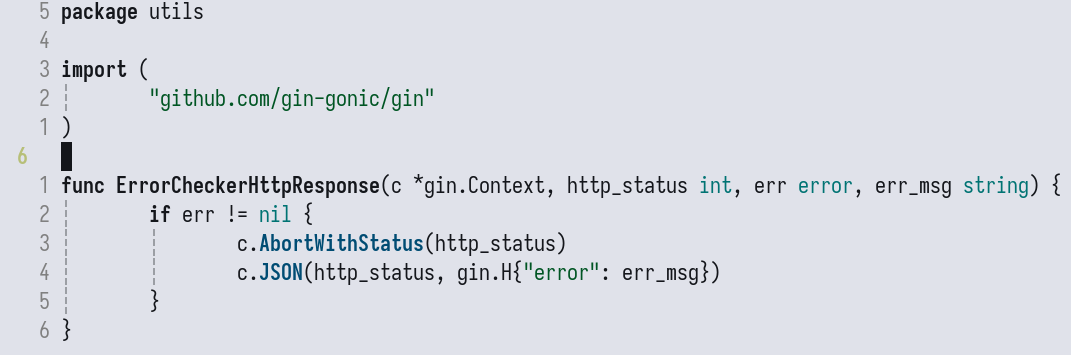
\includegraphics[scale=0.4]{pictures/server_utils.png}
    \caption{Utils layer}
    \label{utilsExample}
\end{figure}

\par
The Models layer contains the structs that represent the entities of the application. 
The structs are used to store the data of the application, and to provide a way to interact with the data.
They also provide a schema of the database, as they are used for mapping the results of the database queries.
Another use for them is to validate the data that is sent to the server, so that we can ensure that the data is correct.

\par
The Database Operations layer contains the functions that interact with the database.
They perform CRUD operations on the database, and to provide the necessary data to the application.
It is the layer that is responsible for the communication between the server and the database.
It's only functionality is the one mentioned above. Other logic, such as validation or error handling, is done elsewhere.
An advantage of writing this layer, instead of choosing and ORM (Object Relational Mapping) library, is that we have more control over the queries that are sent to the database.
This makes the server feel more responsive.

\begin{figure}[htbp]
    \centering
    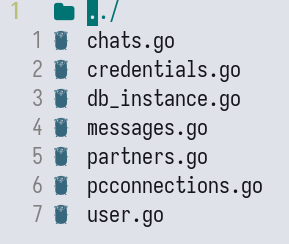
\includegraphics[scale=0.8]{pictures/dboperations.png}
    \caption{Database Operations layer}
    \label{dbOpsExample}
\end{figure}

\par
The Middleware layer goes between the Controllers and the endpoints calls.
It handles the logic that is common to all the endpoints, such as authentication, logging, and error handling.
This makes it easier to add new endpoints, as we don't have to write the same logic for each endpoint.
Also, the handlers for the endpoints can be easily replaced or removed, as they are not tied to the endpoints themselves.

\begin{figure}[htbp]
    \centering
    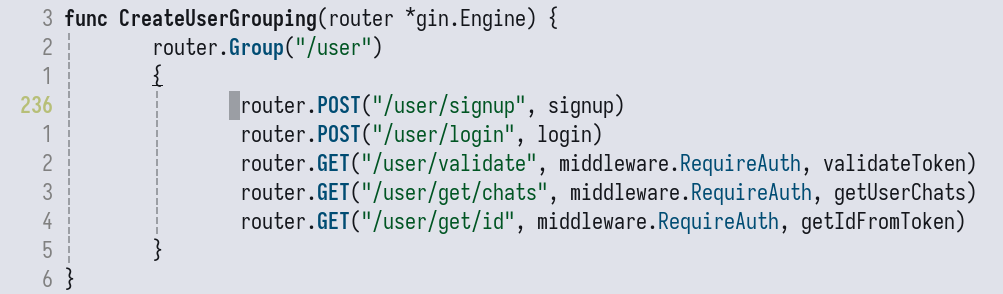
\includegraphics[scale=0.4]{pictures/middleware.png}
    \caption{Middleware layer}
    \label{middlewareExample}
\end{figure}

\par
The Controllers layer contains the functions that handle the requests from the client.
They are used to provide the necessary data to the client, and to handle the data that is sent to the server.
It is the main layer of the server, as they are the ones that interact with the client.
A key point of this layer is that it is not tied to the database, as it only interacts with the Database Operations layer.
I also chose to implement the controllers in a model-based way, as it makes the code more readable and maintainable.

\begin{figure}[htbp]
    \centering
    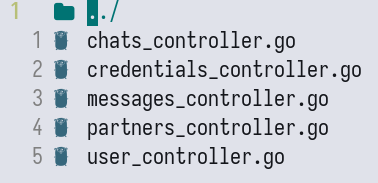
\includegraphics[scale=1.2]{pictures/controllers.png}
    \caption{Controllers layer}
    \label{controllersExample}
\end{figure}

\section{Main focus}
The main entity around which the application is built is the \textit{Partner} class, as seen below.

\begin{figure}[htbp]
    \centering
    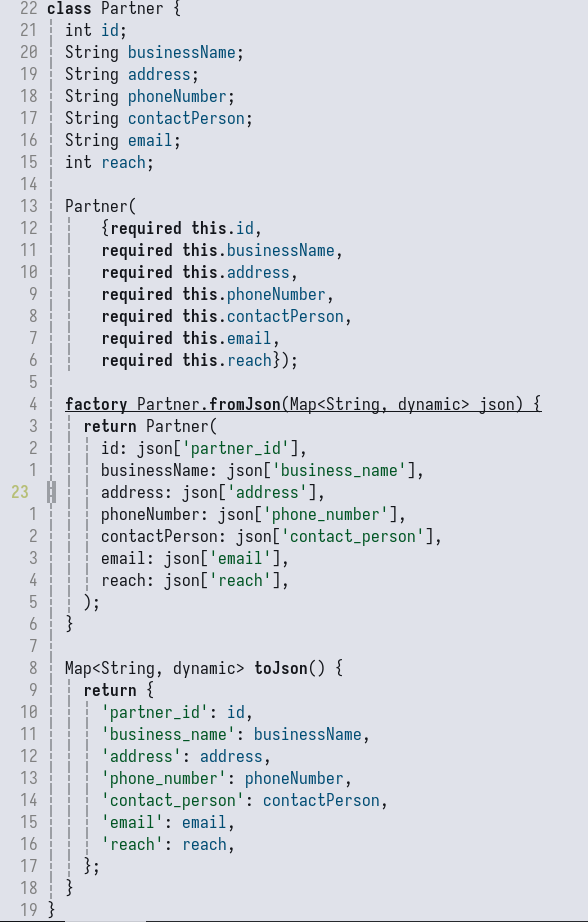
\includegraphics[scale=0.4]{pictures/partner_class.png}
    \caption{Main entity of the application}
    \label{partnersClass}
\end{figure}

This entity is a substitute for the User class, as the User is just a Partner connected with a Credential entity from the DB.
Partner is also connected to the entity Chat, which by itself is connected to Message.
This enforces a good separation of the functionality, and also allows for efficient queries and server responses.
Although this is the main entity, the way it is build, with the additional methods of \textit{fromJson} and \textit{toJson}, allows for easy extension of the application.
This will be present across all the other entities, to manage more easily the bodies of the sent requests.

\par
Now, we'll take a look at how a few components are built, and how their state is managed.
This will contain some good and bad examples, and see how they impact the development of the application, and also the developer experience.

\section{Example Components}
\subsection{Good example}
The first component we'll take a look at is a \textit{Partner list} component. 
To be more specific, the below picture is part of the component that renders the top five partners by reach, a field which represents the average number of clientele.

\begin{figure}[htbp]
    \centering
    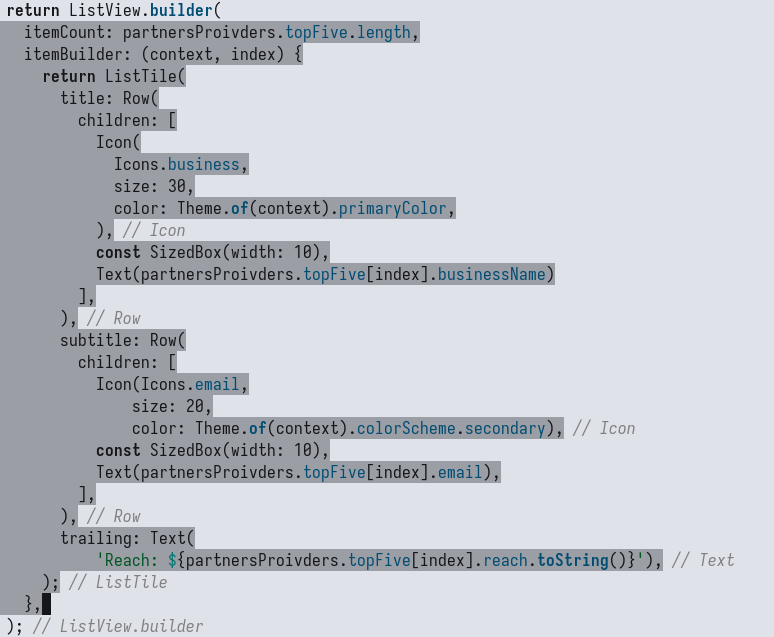
\includegraphics[scale=0.4]{pictures/partners_mapped_good_example.png}
    \caption{List component}
    \label{partnerListComponent}
\end{figure}

Here we can note the good use of states, as the component is stateless, and the state is managed by the provider component.
This is a good practice, as it allows for a more efficient rendering of the component, and also for a more readable code.
Each child sits under a \textit{Consumer} widget, which listens for changes in the provider, and rebuilds the child when the state changes.
By doing so, the component is more efficient, as only the child that needs to be rebuilt is rebuilt, and not the whole component.
Also, it removes for the need of passing the state as a parameter to the child.
Due to the simple nature of the entity is overwatches, it eliminates the need for a websocket.
This is a good example of how to build a component, and how to manage the state of the component, for simple operations on simple entities.

\newpage
\subsection{Bad example}
The second component we'll take a look at is a \textit{Login} component.
This component is used to log in the user, and to provide the necessary data to the application.
In the picture below, we can see that the component is stateful, through the use of controllers.
This is a bad practice, as it makes the component easy to read, but prone to mistakes, due to repetitve coding.

\begin{figure}[htbp]
    \centering
    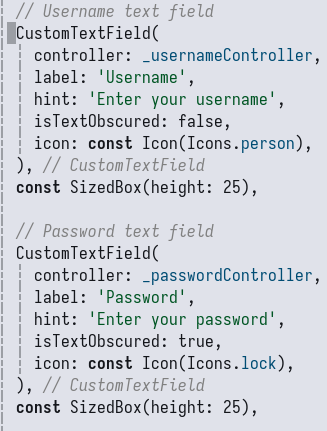
\includegraphics[scale=0.4]{pictures/looks_bad_but_is_good_because.png}
    \caption{Login component}
    \label{loginComponent}
\end{figure}


This is as much avoided as possible, through the makings of custom widgets, that eliminate boilerplate as much as possible.
It is easily observable in the picture below, where \textit{CustomTextField} is used to create a text field, with a custom design, and a custom controller.
Everything under the \textit{Widget build} method would be repeated for each text field, and would make the code harder to read and maintain.
\begin{figure}[htbp]
    \centering
    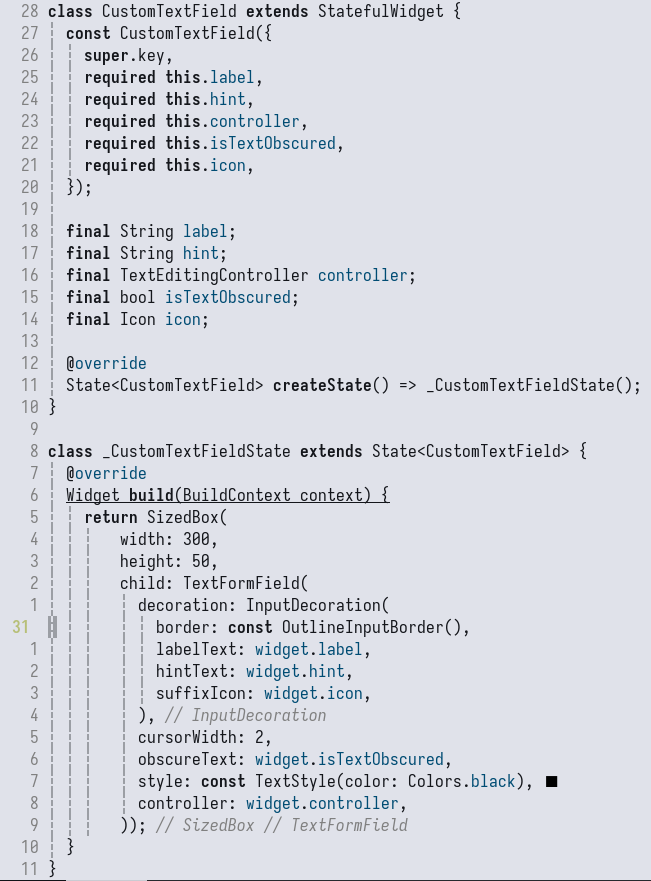
\includegraphics[scale=0.2]{pictures/it_avoid_boilerplate.png}
    \caption{Custom text field}
    \label{customTextField}
\end{figure}



\newpage
\subsection{Neutral example}
The last component we'll take a look at is a \textit{User Details} component.
This component is used to display the details of a user, such as the name, email, and phone number.
It also allows the user to edit the details, and to save the changes.
In the picture below, we can see that the component is stateless, and the state is managed by the \textit{Partners Provider}.

\begin{figure}[htbp]
    \centering
    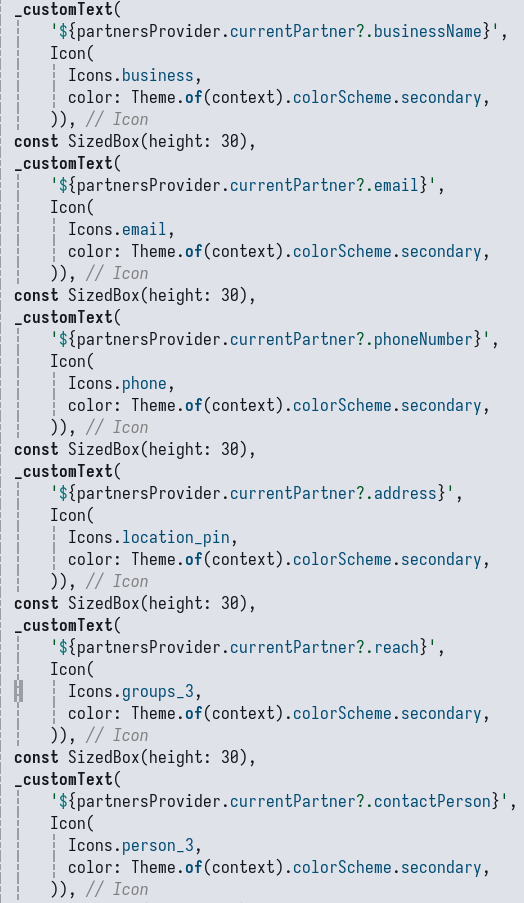
\includegraphics[scale=0.4]{pictures/partners_not_mapped_bad_example.png}
    \caption{User Details component}
    \label{userDetailsComponent}
\end{figure}

This is a bad practice, as it makes the component harder to read, and harder to maintain.
Also, it makes the component less efficient, as there is no need for the whole component to be rebuilt when the provider notifies for changes.
This example, although it is a simple one, shows how not to build a component, and how not to manage the state of the component.
This represents a tricky example, because it looks like a bad mapping, because it is done manually.
In reality, it provides a way to improve the design of the application, by giving custom icons to the inner components.
We can notice this in the picture below.

\begin{figure}[htbp]
    \centering
    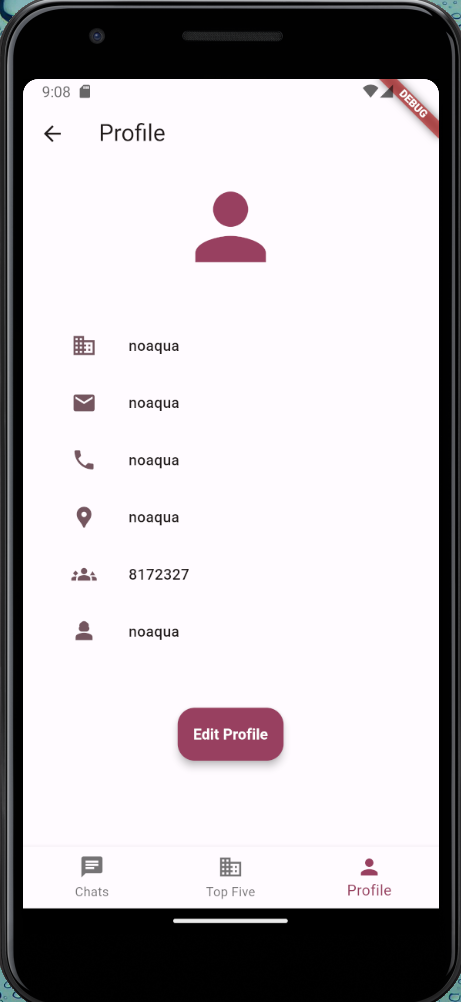
\includegraphics[scale=0.4]{pictures/because_it_looks_bad_we_have_ui.png}
    \caption{User Details UI}
    \label{userDetailsUI}
\end{figure}

\label{implementation}


\chapter{Conclusions}

The research has shown that the use of a cross-platform framework can be beneficial for companies that want to develop applications for multiple platforms.
It can reduce the development time, as the code can be shared between the platforms.
This can also reduce the costs of development, as the developers don't have to learn multiple languages and frameworks.
The research has also shown that the use of a self-implemented server can be beneficial for companies that want to have more control over their data.
It can provide a more realistic scenario, where the data is stored in a company's database, rather than in a third party service.

\par
As noticed in the examples above, the server is separated into different layers, each with its own responsibilities.
The frontend is also separated into different layers, but it requires some manual tweaking in certain use cases.
Both have proven that this separation of concerns can make the code more readable and maintainable, through good and bad examples.
This separation of concerns can also make it easier to add new features to the application, as the code is more organized.

\par
Through the practical implementation of the application, I have learned that the use of a cross-platform framework can be beneficial for companies that want to develop applications for multiple platforms.
Not only that, but the reduction in code duplication can also reduce the development time and costs.
By making use of thoughtful separation of concerns, the code can be more readable and maintainable, and it can be easier to add new features to the application.

\par
It is important to note that the research has some limitations.
The application is developed for Android and Linux devices only, and it uses a self-implemented server.
This means that the application is not available for iOS devices, and it does not use a third party service such as Firebase.
This can limit the reach of the application, as it is not available for all devices.
It can also limit the scalability of the application, as the server is not as robust as a third party service.
But even with these limitations considered, we can still see the benefits of using a cross-platform framework and a self-implemented server, with separation of concerns.


\label{conclusions}

%\addcontentsline{toc}{chapter}{Concluzii}
%\addcontentsline{toc}{chapter}{Conclusions}

\bibliography{references}

\end{document}

